%%%%%%%%%%%%%%%%%%%%%%%%%%%%%%%%%%%%%%%%%%%%%%%%%%%%%%%%%%%%%%%%%%%%%%
% Lớp 11 | Đường thẳng, mặt phẳng. Quan hệ song song trong | Hai mặt phẳng song song
% Dạng 1H4?4-4: Xác định mặt phẳng đi qua một điểm và song song với một mặt phẳng
% Số câu: 33  (sinh tự động bởi tach_cau.py; từ nay thầy sửa trực tiếp file này)
%%%%%%%%%%%%%%%%%%%%%%%%%%%%%%%%%%%%%%%%%%%%%%%%%%%%%%%%%%%%%%%%%%%%%%

%%%%%%%%%%%%%%%% TRẮC NGHIỆM 4 PHƯƠNG ÁN %%%%%%%%%%%%%%%%

% nguồn: Ok_Toan11_TracNghiem_Lan2
\begin{ex}%[1H4H4-4]%[ma:1b57c1f7]
	Cho hình vuông $ABCD$ và tam giác đều $SAB$ nằm trong hai mặt phẳng khác nhau. Gọi $M$ là điểm di động trên đoạn $A B$ ($ M  $ khác $ A $ và $ B $). Mặt phẳng $(\alpha)$ qua $M$ song song với $(SBC)$ cắt hình chóp $S.ABCD$ theo thiết diện là
	\choice 
		{Hình  tam giác}
		{Hình  vuông}
		{Hình bình hành} 
		 {\True Hình thang}
	 \loigiai{
		\begin{center}
			\begin{tikzpicture}[scale=0.7,font=\footnotesize,line join=round,line cap=round,>=stealth]
					\coordinate (A)  at (0,0);
					\coordinate (D) at  (-2,-3);
					 \coordinate (B) at (7,0);
					\coordinate (C) at  ($(B)+(D)-(A)$);
					 \coordinate (S) at ($(A)+(0.5,5)$);
					\coordinate (M)  at ($(A)!0.5!(B)$);
					\coordinate  (N) at ($(C)!0.5!(D)$);
					\coordinate (P) at  ($(S)!0.5!(D)$);
					\coordinate (Q)  at ($(S)!0.5!(A)$);
					\fill[yellow](M)--(N)--(P)--(Q)--cycle; 
					 \draw (S)--(B)
						 (S)--(C)
						 (S)--(D)
						(B)--(C)--(D) 
						 (P)--(N);
					\draw[dashed](S)--(A) 
						(A)--(B) 
						 (A)--(D)
						(A)--(C) 
						 (B)--(D)
						 (N)--(M)--(Q)--(P);
					\foreach \i/\g in {S/90,A/45,B/-90,C/-90,D/-90,M/45,N/-90,P/180,Q/180}{\draw[fill=black](\i) circle (1pt) 
						($(\i)+(\g:3mm)$) node[scale=1]{$\i$};} 
				\end{tikzpicture}
		\end{center}
		Do $(\alpha)\parallel (SBC)$  nên $(\alpha)$ cắt mặt phẳng $(A B C D)$ theo giao tuyến $M N\parallel BC$, $(N\in CD)$.\\
		Hoàn toàn tương tự, ta có $(\alpha)$ cắt các mặt phẳng $(SAB)$ và $(SCD)$ theo các giao tuyến $MQ$, $NP$ ở đó $Q \in S A$  và $MQ\parallel SB$; $P \in SD$ và $N P\parallel SC$.\\
		Mặt phẳng $(\alpha)$ cắt hình chóp $S.ABCD$ theo thiết diện là tứ giác $MNPQ$.\\ 
	Dễ thấy $PQ \parallel AD$, $PQ\neq A D$ từ  đó suy ra $MNPQ$ là hình thang.}
\end{ex}

% nguồn: Ok_Toan11_TracNghiem_Lan2
\begin{ex}%[1H4H4-4]%[ma:c891c906]
	Cho hình hộp $ABCD.A'B'C'D'$. Gọi $I$ là trung điểm của cạnh $AB$, $(\alpha)$ là mặt  phẳng đi qua $I$ và song song với mặt phẳng $\left(BDD'\right)$. Thiết diện của hình hộp cắt bởi mặt phẳng $(\alpha)$ là hình gì?
	 \choice
		{Hình tam giác} 
		{\True Hình  bình hành}
		{Hình ngũ giác} 
		{Hình thang} 
	\loigiai{ 
		\begin{center}
			\begin{tikzpicture}[scale=0.7,font=\footnotesize,line join=round,line cap=round,>=stealth]
					\coordinate (A')  at (0,0);
					\coordinate (B') at  (-2,-2);
					\coordinate (C') at  (5,-2);
					 \coordinate (D') at (7,0);
					\coordinate (A) at  ($(A')+(0,5)$);
					\coordinate (B)  at ($(B')+(0,5)$);
					\coordinate (C) at ($(C')+(0,5)$); 
					\coordinate  (D) at ($(D')+(0,5)$);
					\coordinate (I) at ($(A)!0.5!(B)$); 
					\coordinate (I')  at ($(A')!0.5!(B')$);
					\coordinate (K')  at ($(A')!0.5!(D')$);
					\coordinate (K) at  ($(A)!0.5!(D)$);
					\fill[yellow](I)--(K)--(K')--(I')--cycle; 
					\draw (A)--(B)--(C)--(D)--cycle  (B)--(B')--(C')--(C)
						 (C')--(D')--(D)
						 (I)--(K)
						 (B)--(D);
					\draw[dashed] (B')--(A')--(D') 
						(A')--(A) 
						 (I)--(I')--(K')--(K)
						 (B')--(D');
					\foreach \i/\g in {A'/-90,B'/-90,C'/-45,D'/0,A/90,B/180,C/90,D/0,I'/180,I/180,K/90,K'/-90}{\draw[fill=black](\i)  circle (1pt)
						($(\i)+(\g:3mm)$)  node[scale=1]{$\i$};}
				\end{tikzpicture}
		\end{center}
		Qua $I$  kẻ đường thẳng song song với $BD$ cắt $A D$ tại $K$.\\
		Qua $K$ kẻ đường thẳng song song với $DD'$ cắt $A'D'$  tại $K'$.\\
		Qua $I$ kẻ đường thẳng song song với $BB'$ cắt $A'B'$ tại $I'$.\\ 
		Thiết diện cần tìm là hình bình  hành $IKK'I'$.
	} 
\end{ex}

% nguồn: Ok_Toan11_TracNghiem_Lan2
\begin{ex}%[1H4H4-4]%[ma:cdb085ec]
	Cho tứ diện đều $S.ABC$. Gọi $I$ là trung điểm của đoạn $A B$, $M$ là điểm di động trên đoạn $A I$. Qua $M$ vẽ mặt phẳng $(\alpha)$ song song với $(SIC)$. Thiết  diện tạo bởi $(\alpha)$ với tứ diện $S.ABC$ là
	\choice 
		{\True  Tam giác cân tại $M$}
		{Hình  bình hành}
		 {Tam giác đều}
		 {Hình thoi}
	\loigiai{ 
		\begin{center}
			\begin{tikzpicture}[scale=0.7,font=\footnotesize,line join=round,line cap=round,>=stealth]
					\coordinate (S) at (0,4); 
					\coordinate (A)  at (-2,0);
					 \coordinate (B) at (0,-3);
					\coordinate (C) at  (5,0);
					\coordinate  (I) at ($(A)!0.5!(B)$);
					\coordinate (M) at  ($(I)!0.45!(A)$);
					\coordinate  (N) at ($(C)!0.45!(A)$);
					 \coordinate (P) at ($(S)!0.45!(A)$);
					 \fill[yellow](M)--(N)--(P)--cycle;
					 \draw (S)--(A)
						(S)--(B) 
						 (S)--(C)
						(B)--(C) 
						(A)--(B) 
						 (M)--(P)
						(S)--(I); 
					\draw[dashed](A)--(C) 
						 (M)--(N)--(P)
						 (I)--(C);
					\foreach \i/\g in {S/90,A/180,B/-90,C/0,M/180,N/45,P/120,I/220}{\draw[fill=black](\i)  circle (1pt)
						 ($(\i)+(\g:3mm)$) node[scale=1]{$\i$};}
				\end{tikzpicture}
		\end{center}
		Trong mặt phẳng $(SAB)$  qua $M$ kẻ đường thẳng song song với $SI$ cắt $SA$ tại $P$.\\
		Trong mặt phẳng $(ABC)$  qua $M$ kẻ đường thẳng song song với $IC$ cắt $AC$ tại $N$.\\
		 Thiết diện là tam giác $MNP$.\\
		Ta có $\dfrac{MP}{SI}=\dfrac{MN}{CI}\Rightarrow MP=MN$ (vì $SI=CI)$.\\ 
		Vậy thiết  diện là tam giác $MNP$ cân tại $M$.
	 }
\end{ex}

% nguồn: Ok_Toan11_TracNghiem_Lan2
\begin{ex}%[1H4H4-4]%[ma:fc14aad2]
	Cho hình chóp $S.ABCD$ có đáy $ABCD$ là hình bình hành tâm $O$. Gọi $M$ là điểm bất kì không trùng với $ S $ trên đoạn  thẳng $SO$. Mặt phẳng $(\alpha)$ qua $M$ và song song với $(ABCD)$. Thiết diện của hình chóp $S.ABCD$ cắt bởi mặt phẳng $(\alpha)$ là hình gì?
	\choice 
		{\True Hình  bình hành}
		{Hình tam  giác}
		{Hình ngũ  giác}
		 {Hình thang cân}
	 \loigiai{
		\begin{center}
			\begin{tikzpicture}[scale=0.7,font=\footnotesize,line join=round,line cap=round,>=stealth]
					\coordinate (A) at  (0,0);
					\coordinate  (D) at (-2,-3);
					\coordinate  (B) at (7,0);
					\coordinate  (C) at ($(B)+(D)-(A)$);
					\coordinate (S) at  ($(A)+(0.5,5)$);
					\coordinate (O) at  ($(A)!0.5!(C)$);
					\coordinate (E)  at ($(S)!0.7!(A)$);
					 \coordinate (H) at ($(S)!0.7!(D)$);
					\coordinate  (G) at ($(S)!0.7!(C)$);
					\coordinate  (F) at ($(S)!0.7!(B)$);
					 \coordinate (M) at ($(E)!0.5!(G)$);
					\fill[yellow](E)--(H)--(G)--(F)--cycle; 
					\draw (S)--(B) 
						 (S)--(C)
						(S)--(D) 
						 (B)--(C)--(D)
						 (H)--(G)--(F);
					 \draw[dashed](S)--(A)
						 (A)--(B)
						(A)--(D) 
						 (A)--(C)
						(B)--(D) 
						 (H)--(E)--(F)
						 (E)--(G)
						(H)--(F) 
						 (S)--(O);
					\foreach \i/\g in {S/90,A/45,B/-90,C/-90,D/-90,O/-90,H/180,E/45,M/-120,F/45,G/0}{\draw[fill=black](\i) circle  (1pt)
						($(\i)+(\g:3mm)$) node[scale=1]{$\i$};} 
				\end{tikzpicture}
		\end{center}
		Xét mặt phẳng $(SAC)$ và mặt phẳng $(\alpha)$ có $M$ là điểm chung và $AC\parallel(\alpha)$ nên giao tuyến là đường thẳng đi qua $M$ và song song với $AC$ cắt $SA$, $SC$ lần lượt tại $E$, $G$.\\ 
		Tương  tự $(\alpha)$ cắt $SB$, $SD$ lần lượt tại $F$, $H$. \\
		Khi đó thiết diện  cần tìm là tứ giác $EFGH$.\\
		Ta có $EF\parallel G H$  và $FG\parallel EH$ nên thiết diện là hình bình hành.
	 }
\end{ex}

% nguồn: Ok_Toan11_TracNghiem_Lan2
\begin{ex}%[1H4V4-4]%[ma:ab2d7d30]
	Cho hình chóp $S.ABCD$ có đáy $ABCD$ là hình bình hành. Gọi $M$, $N$, $P$ lần lượt là trung điểm của $AB$, $AD$, $BC$, điểm $I$ thuộc cạnh $SA$ thỏa mãn $SI=3IA$. Mặt phẳng $(\alpha)$ đi qua $P$ và song song với mặt phẳng $(IMN)$ cắt  hình chóp theo một thiết diện là hình gì?
	\choice 
		 {Tứ giác}
		{\True Ngũ giác} 
		{Lục giác} 
		{Tam giác} 
	 \loigiai{
		\begin{center}
			\begin{tikzpicture}[scale=1,font=\footnotesize,line join=round,line cap=round,>=stealth]
					\def\a{2.9}  \def\b{2.2} \def\c{6} \def\d{3.9} \def\e{6}
					\path  (0,0) coordinate (D)
						(\a,\b)  coordinate (A)
						(\c,0)  coordinate (C)
						(\d,\e) coordinate (S) 
						($(A)+(C)-(D)$)  coordinate (B)
						($(S)!.5!(B)$) coordinate (H) 
						($(S)!.5!(D)$) coordinate  (F)
						($(A)!.5!(C)$)  coordinate (O)
						($(O)!.5!(C)$) coordinate  (Q)
						 ($(D)!.5!(C)$) coordinate (E)
						($(B)!.5!(C)$) coordinate  (P)
						 ($(A)!.5!(O)$) coordinate (K)
						($(A)!.5!(D)$) coordinate (N) 
						 ($(A)!.5!(B)$) coordinate (M)
						 ($(A)!.25!(S)$) coordinate (I)
						($(A)!.75!(S)$)  coordinate (G);
					\draw  (S)--(D)--(C)--(B)--(S)--(C)--(E)--(F)
						(P)--(H); 
					\draw[dashed] (S)--(A)--(D)--(B)--(A)--(C) 
						 (E)--(P)
						 (K)--(I)--(M)--(N)--(I)
						(F)--(G)--(H) 
						(G)--(Q); 
					\foreach \d/\g in {S/90,A/180,B/0,C/-90,D/-90,E/-90,F/180,G/45,H/60,P/-60,Q/-90,O/-90,K/-90,I/45,N/-60,M/90} 
					 \draw[fill=black] (\d) circle (1pt) +(\g:3mm) node{$\d$};
				\end{tikzpicture}
		\end{center}
		$P$ là một điểm chung của $(\alpha)$ và mặt phẳng $(ABCD)$ nên giao tuyến của $(\alpha)$ và mặt phẳng $(ABCD)$ là đường thẳng đi qua  $P$ và song song với $MN$, giao tuyến này cắt $CD$ và $AC$ lần lượt tại $E$ và $Q$.\\
		Trong mặt phẳng $(ABCD)$, gọi $K$ là giao  điểm của $AC$ và $MN$.\\
		$Q$ là một điểm chung của $(\alpha)$ và mặt phẳng $(SAC)$ nên giao tuyến của $(\alpha)$ và mặt phẳng $(SAC)$ là đường thẳng đi qua $Q$ và song song với $IK$, giao tuyến này cắt $SA$ tại  $G$.\\
		$G$ là một điểm chung của $(\alpha)$ và mặt phẳng $(SAB)$ nên giao tuyến của $(\alpha)$ và mặt phẳng $(SAB)$ là đường thẳng đi qua $G$ và song song với $IM$,  giao tuyến này cắt $SB$ tại $H$.\\
		$G$ là một điểm chung của $(\alpha)$ và mặt phẳng $(SAD)$ nên giao tuyến của $(\alpha)$ và mặt phẳng $(SAD)$  là đường thẳng đi qua $G$ và song song với $IN$, giao tuyến này cắt $SD$ tại $F$.\\
		Vậy thiết diện của hình chóp khi cắt  bởi $\mathrm{mp}(\alpha)$ là ngũ giác $EFGHP$.
	 }
\end{ex}

% nguồn: Ok_Toan11_TracNghiem_Lan2
\begin{ex}%[1H4V4-4]%[ma:0f306d25]
	Cho hình chóp $S.ABCD$ có đáy $A B C D$ là hình bình hành tâm $O$, $A B=8$, $SA=SB=6$. Gọi $(P)$ là mặt phẳng đi qua $O$ và song song với $(SAB)$. Tính diện tích của thiết diện của  $(P)$ và hình chóp $S.A B C D$.
	\choice 
		{$12$} 
		{$5  \sqrt{5}$}
		{$6  \sqrt{5}$}
		{\True $13$} 
	\loigiai{ 
		\begin{center}
			\begin{tikzpicture}[scale=1,font=\footnotesize,line join=round,line cap=round,>=stealth]
					\coordinate (A) at (0,0); 
					 \coordinate (D) at (-2,-3);
					 \coordinate (B) at (7,0);
					 \coordinate (C) at ($(B)+(D)-(A)$);
					\coordinate (S) at ($(A)+(1,5)$); 
					 \coordinate (O) at ($(A)!0.5!(C)$);
					\coordinate (N)  at ($(S)!0.5!(D)$);
					 \coordinate (M) at ($(S)!0.5!(C)$);
					\coordinate (Q) at ($(B)!0.5!(C)$); 
					\coordinate (P)  at ($(A)!0.5!(D)$);
					\coordinate (H) at ($(Q)!0.85!(O)$); 
					\fill[yellow](M)--(N)--(P)--(Q)--cycle; 
					\draw (S)--(B) 
						 (S)--(C)
						(S)--(D) 
						 (B)--(C)--(D)
						(N)--(M)--(Q); 
					 \draw[dashed](S)--(A)
						(A)--(B) 
						 (A)--(D)
						(A)--(C) 
						(B)--(D) 
						 (N)--(P)--(Q)
						(M)--(H); 
					 \foreach \i/\g in {S/90,A/45,B/-90,C/-90,D/-90,O/-90,Q/0,M/45,N/180,P/-90,H/-60}{\draw[fill=black](\i) circle (1pt)
						 ($(\i)+(\g:3mm)$) node[scale=1]{$\i$};}
				\end{tikzpicture}
		\end{center}
		Qua $ O  $ dựng đường thẳng song song với $ AB $, cắt $ AD $ và $ BC $ lần lượt tại $ P $ và $ Q $.\\
		Khi đó $P$,  $Q$ lần lượt là trung điểm của $AD$ và $B C$.\\
		Qua $ P $ dựng đường thẳng song song với $ SA $, cắt $ SD  $ tại $ N $.\\
		$\Rightarrow N$ là trung điểm của  $SD$.\\
		Qua $Q$ dựng đường thẳng song song với $ SB  $, cắt $ SC $ tại $ M $.\\
		$\Rightarrow  M$ là trung điểm của $SC$.\\
		Nối $M$ và $N$ ta có thiết diện của $(P)$ và hình chóp $S.ABCD$ là tứ giác $M N P  Q$.\\
		Vì $P Q \parallel C D$, $M N \parallel CD$ nên $PQ \parallel MN$  nên tứ giác $MNPQ$ là hình thang.\\
		Ta có $\heva{&PQ=A B=8\\&M N=\dfrac{1}{2}AB=4\\ &MQ=NP=\dfrac{1}{2}SA=3}$ $\Rightarrow MNPQ$ là hình thang  cân.\\
		Gọi $H$ là  chân đường cao hạ từ đỉnh $M$ của hình thang $MNPQ$.\\
		Khi đó ta có  $HQ=\dfrac{1}{4}PQ=2\Rightarrow MH=\sqrt{MQ^2-HQ^2}=\sqrt{5}$.\\
		 Vậy diện tích của thiết diện cần tìm là
		\[S=\dfrac{(M N+P Q) \cdot  M H}{2}=6 \sqrt{5}.\]
	} 
\end{ex}

% nguồn: Ok_Toan11_TracNghiem_Lan2
\begin{ex}%[1H4V4-4]%[ma:15df6734]
	Cho hình hộp $A B C D.A'B'C'D'$ và điểm $M$ nằm giữa hai điểm $A$ và $B$. Gọi $(P)$  là mặt phẳng đi qua $M$ và song song với mặt phẳng $(AB'D')$. Mặt phẳng $(P)$ cắt hình hộp theo thiết diện là hình gì?
	\choice 
		{Hình tứ  giác}
		{Hình tam  giác}
		{\True Hình  lục giác}
		{Hình ngũ  giác}
	 \loigiai{
		\begin{center}
			\begin{tikzpicture}[scale=0.7,font=\footnotesize,line join=round,line cap=round,>=stealth]
					\coordinate (A') at (0,0); 
					\coordinate (B') at (-2,-2); 
					\coordinate (C') at  (5,-2);
					\coordinate (D')  at (7,0);
					\coordinate  (A) at ($(A')+(0,5)$);
					\coordinate  (B) at ($(B')+(0,5)$);
					\coordinate (C) at ($(C')+(0,5)$); 
					\coordinate  (D) at ($(D')+(0,5)$);
					 \coordinate (M) at ($(A)!0.4!(B)$);
					 \coordinate (H) at ($(A)!0.4!(D)$);
					\coordinate (G) at  ($(D')!0.4!(D)$);
					 \coordinate (Q) at ($(D')!0.4!(C')$);
					 \coordinate (P) at ($(B')!0.4!(C')$);
					\coordinate  (N) at ($(B')!0.4!(B)$);
					 \fill[yellow](M)--(H)--(G)--(Q)--(P)--(N)--cycle;
					\draw (A)--(B)--(C)--(D)--cycle (B)--(B')--(C')--(C) 
						 (C')--(D')--(D)
						 (M)--(H)
						 (G)--(Q)
						 (B)--(D)
						(B)--(C'); 
					\draw[dashed]  (B')--(A')--(D')
						 (A')--(A)
						(B')--(D') 
						 (M)--(N)--(P)--(Q)
						 (H)--(G)
						 (B')--(A)--(D');
					\foreach \i/\g in  {A'/-90,B'/-90,C'/-45,D'/0,A/90,B/180,C/135,D/0,M/180,H/90,G/0,Q/-45,P/-90,N/180}{\draw[fill=black](\i) circle (1pt)
						($(\i)+(\g:3mm)$) node[scale=1]{$\i$};} 
				\end{tikzpicture}
		\end{center}
		Ta có  $ \heva{&BC' \parallel AD'\\&BD\parallel B'D'\\&BC',BD\subset(BC'D)\\&AD',BD'\subset (AB'D')\\&BC'\cap BD=\{B\}} \Rightarrow\left(BC'D\right) \parallel\left(AB'D'\right)\parallel(P)$ $\quad (1)$.\\
		Do $(1)$ ta giả sử $(P)$ cắt  $BB'$ tại $N$ suy ra $(P) \cap\left(ABB'A'\right)=MN$.\\
		Mà $\left(AB'D'\right)\cap\left(ABB'A'\right)=AB'$ suy ra $M N \parallel AB'$.  \\
		Do đó $N$ thuộc  cạnh $BB'$.\\
		Tương tự  giả sử $(P) \cap B'C'=P$ suy ra $(P) \cap\left(B C C'B'\right)=NP$.\\
		Kết hợp với (1) suy ra $N P  \parallel BC'$.\\
		Tương tự $(P) \cap C'D'=Q$ sao cho $P Q \parallel B'D'$; $(P) \cap DD'=G$  sao cho $Q G \parallel C'D$.\\
		Hơn nữa $(P) \cap AD=H$ sao  cho $G H \parallel AD'$.\\
		Từ đó  suy ra thiết diện là lục giác $MNPQGH$.
	 }
\end{ex}

% nguồn: Ok_Toan11_TracNghiem_Lan2
\begin{ex}%[1H4V4-4]%[ma:e9a006d0]
	Cho tứ diện đều $ABCD$ cạnh $a$ và $G$ là trọng tâm tam giác $ABC$. Cắt tứ diện bởi mặt phẳng $(P)$ qua $G$ và song song với mặt phẳng  $(BCD)$ thì diện tích thiết diện bằng bao nhiêu?
	\choice 
		{\True  $\dfrac{a^2\sqrt{3}}{16}$}
		 {$\dfrac{a^2\sqrt{3}}{4}$}
		 {$\dfrac{a^2\sqrt{3}}{9}$}
		 {$\dfrac{a^2\sqrt{3}}{18}$}
	\loigiai{\begin{center}
		\begin{tikzpicture}[scale=0.7,font=\footnotesize,line join=round,line cap=round,>=stealth]
				\coordinate  (A) at (0,4);
				\coordinate  (B) at (-2,0);
				\coordinate (C) at (0,-3); 
				\coordinate (D) at (5,0); 
				\coordinate (K)  at ($(A)!0.6!(B)$);
				\coordinate (H) at ($(A)!0.6!(C)$); 
				\coordinate  (I) at ($(A)!0.6!(D)$);
				\coordinate (M) at  ($(B)!0.5!(C)$);
				 \coordinate (G) at ($(A)!0.6!(M)$);
				 \fill[yellow](K)--(H)--(I)--cycle;
				\draw (A)--(B)--(C)--cycle (C)--(D)--(A) 
					(A)--(M) 
					(K)--(H)--(I); 
				\draw[dashed] (K)--(I) 
					(B)--(D); 
				\foreach \i/\g in {A/90,B/180,C/-90,D/0,K/180,H/-45,I/45,G/220,M/-135}{\draw[fill=black](\i)  circle (1pt)
					 ($(\i)+(\g:3mm)$) node[scale=1]{$\i$};}
			\end{tikzpicture}
	\end{center}
	Trong mặt phẳng $(ABC)$ kẻ đường thẳng qua $G$ và song song với $B C$ cắt $A C$, $A B$ lần lượt tại  $H$, $K$.\\
	Trong mặt phẳng $(ACD)$ kẻ đường thẳng qua $H$  và song song với $CD$ cắt $AD$ tại $I$.\\
	Thiết diện cần tìm là tam giác  $KHI$.\\
	Ta có $ KH $, $ KI $, $ HI $ lần lượt song song với  $ BC $, $ BD $, $ CD $ nên
	$$ \dfrac{KH}{BC}=\dfrac{AK}{AB}=\dfrac{KI}{BD}=\dfrac{AI}{AD}=\dfrac{HI}{CD}.  $$
	Mà $ BC=BD=CD $ nên $ HK=KI=HI $ nên tam giác $ HKI $ là tam  giác đều.\\
	 Hơn nữa, ta có với $ HK \parallel BC $ nên $ \dfrac{HK}{BC}=\dfrac{AG}{AM}=\dfrac{2}{3} \Rightarrow HK=\dfrac{2}{3}BC=\dfrac{2}{3}a$.\\
	Do đó  $S_{KHI}=\dfrac{HK^2\cdot \sqrt{3}}{4}= \dfrac{\left(\tfrac{2}{3}a\right)^2\cdot \sqrt{3}}{4}=\dfrac{a^2 \sqrt{3}}{9}$.
} 
\end{ex}

% nguồn: Ok_Toan11_TracNghiem_Lan2
\begin{ex}%[1H4V4-4]%[ma:b7e8e914]
	Cho hình chóp $S.ABCD$ có đáy $ABCD$ là hình bình hành tâm $O$. Tam giác $SBD$ đều. Một mặt phẳng $(P)$ song song với $(SBD)$ và qua điểm $I$ thuộc cạnh $AC$ (không trùng với $A$ hoặc $C$). Thiết diện của $(P)$ và hình chóp là hình  gì?
	 \choice
		{Hình  bình hành}
		{\True Tam giác đều} 
		{Tam giác  vuông}
		{Tam giác cân không  đều}
	 \loigiai{
		\begin{center}
			\begin{tikzpicture}[scale=0.7,font=\footnotesize,line join=round,line cap=round,>=stealth]
					\coordinate (A) at (0,0); 
					\coordinate (D) at (-2,-3); 
					\coordinate  (B) at (7,0);
					\coordinate (C) at  ($(B)+(D)-(A)$);
					 \coordinate (S) at ($(A)+(1,5)$);
					\coordinate (O) at  ($(A)!0.5!(C)$);
					\coordinate (I)  at ($(A)!0.3!(O)$);
					\coordinate  (E) at ($(S)!0.5!(C)$);
					\coordinate (M) at ($(C)!0.5!(D)$); 
					\coordinate (N) at ($(C)!0.5!(B)$); 
					 \fill[yellow](M)--(N)--(E)--cycle;
					\draw  (S)--(B)
						 (S)--(C)
						 (S)--(D)
						(B)--(C)--(D) 
						 (N)--(E)--(M);
					 \draw[dashed](S)--(A)
						 (A)--(B)
						 (A)--(D)
						 (A)--(C)
						 (B)--(D)
						 (M)--(N)--(E)
						(S)--(O); 
					\foreach \i/\g in {S/90,A/180,B/-90,C/-90,D/-90,O/-90,N/-90,M/-90,E/45,I/-90}{\draw[fill=black](\i) circle  (1pt)
						($(\i)+(\g:3mm)$)  node[scale=1]{$\i$};}
				\end{tikzpicture}
		\end{center}
		\begin{itemize}
			\item \textbf{Trường hợp 1:} Điểm  $I$ thuộc đoạn $O C$. \\
			Gọi $M$, $N$, $E$ lần lượt là giao  điểm của $(P)$ với các đường thẳng $C D$, $BC$, $S C$.\\
			Ta có thiết diện của $(P)$ và hình  chóp là tam giác $EMN$.\\
			Ta có $\heva{&(P)\parallel(SBD)\\&(ABCD)\cap(SBD)=BD\\&(P)\cap(ABCD)=MN}\Rightarrow MN\parallel BD\Rightarrow  \dfrac{MN}{BD}=\dfrac{CM}{CD}=t\Rightarrow MN=t\cdot BD$.\\
			Ta lại  có $\heva{&(P)\parallel(SBD)\\&(SCD)\cap(SBD)=SD\\&(P)\cap(SCD)=ME}\Rightarrow ME\parallel SD\Rightarrow \dfrac{ME}{SD}=\dfrac{CM}{CD}=t\Rightarrow ME=t\cdot SD$.\\
			Tương tự $EN \parallel SB$ và $EN=t\cdot SB$.\\ 
			 Mà $SB=BD=SD$ nên $MN=EM=EN$.\\
			Suy ra tam giác $MNE$ là  tam giác đều.
			\item \textbf{Trường hợp 2:} Điểm $I$ thuộc $O A$.  Làm tương tự như trên ta được thiết diện của $(P)$ và hình chóp cũng là một tam giác dều.
		\end{itemize}
	 }
\end{ex}

% nguồn: Ok_Toan11_TracNghiem_Lan2
\begin{ex}%[1H4V4-4]%[ma:c0176001]
	Cho hình chóp $S.ABCD$ có đáy là hình vuông tâm $O$, cạnh $a$, các cạnh bên đều bằng $2a$. Gọi $(\alpha)$ là mặt phẳng đi qua $O$ và song song với mặt phẳng $(SBC)$. Tính chu vi $P$ của thiết diện tạo bởi mặt phẳng  $(\alpha)$ và hình chóp $S.ABCD$.
	\choice 
		{\True $P=\dfrac{7 a}{2}$} 
		{$P=\dfrac{11 a}{2}$} 
		{$P=\dfrac{9  a}{2}$}
		{$P=\dfrac{5  a}{2}$}
	\loigiai{ 
		\begin{center}
			\begin{tikzpicture}[scale=0.7,font=\footnotesize,line join=round,line cap=round,>=stealth]
					 \coordinate (A) at (0,0);
					\coordinate  (D) at (-2,-3);
					\coordinate (B) at (7,0); 
					\coordinate (C) at ($(B)+(D)-(A)$); 
					\coordinate (S)  at ($(A)+(0.5,5)$);
					 \coordinate (M) at ($(A)!0.5!(B)$);
					\coordinate (N) at ($(C)!0.5!(D)$); 
					 \coordinate (P) at ($(S)!0.5!(D)$);
					\coordinate (Q)  at ($(S)!0.5!(A)$);
					\coordinate (O) at ($(C)!0.5!(A)$); 
					\fill[yellow](M)--(N)--(P)--(Q)--cycle; 
					\draw (S)--(B) 
						(S)--(C) 
						 (S)--(D)
						(B)--(C)--(D) 
						(P)--(N); 
					 \draw[dashed](S)--(A)
						(A)--(B) 
						(A)--(D) 
						 (N)--(M)--(Q)--(P);
					\foreach \i/\g  in {S/90,A/45,B/-90,C/-90,D/-90,M/45,N/-90,P/180,Q/180,O/-90}{\draw[fill=black](\i) circle (1pt)
						 ($(\i)+(\g:3mm)$) node[scale=1]{$\i$};}
				\end{tikzpicture}
		\end{center}
		Do $(\alpha)\parallel(SBC)$ nên $(\alpha)$ cắt mặt phẳng $(ABCD)$ theo giao tuyến đi qua $O$ song song  với $B C$ và cắt $A B$ tại $M$, cắt $C D$ tại $N$.\\
		Hoàn toàn tương tự ta có $(\alpha)$ cắt  các mặt phẳng $(SAB)$ và $(SCD)$ theo các giao tuyến $MQ$, $NP$ ở đó $Q \in SA$ và $M Q \parallel SB$; $P \in SD$ và $NP\parallel SC$.\\
		Mặt phẳng $(\alpha)$ cắt hình chóp $S.ABCD$ theo thiết  diện là tứ giác $MNPQ$.\\
		Lại có $O$ là trung điểm $AC$ nên $M$, $N$, $P$, $Q$ lần lượt là trung điểm của $A B$, $C  D$, $S D$, $SA$.\\
		 Suy ra $MN=a$, $NP=\dfrac{1}{2}SC=a, MQ=\dfrac{1}{2}SB=a$, $PQ=\dfrac{1}{2} AD=\dfrac{a}{2}$.\\
		Vậy chu  vi của thiết diện là \[P=MN+NP+PQ+QM=a+a+\dfrac{a}{2}+a=\dfrac{7a}{2}.\]
	 }
\end{ex}

% nguồn: Ok_TracNghiemLop11_Lan1
\begin{ex}%[1H4V4-4]%[ma:ac0097be]
	Cho hình chóp $S.ABCD$ có đáy $ABCD$ là hình  bình hành, mặt bên $SBC$ là tam giác đều. Gọi $M$ là điểm di động trên đoạn thẳng $AB$, ($M\ne A;M\ne B$). Qua $M$ dựng mặt phẳng $(\alpha)$ song song với mặt phẳng $(SBC)$. Thiết diện tạo với mặt phẳng $(\alpha)$ và chóp $S.ABCD$ là hình gì?
	 \choice
		{\True Hình thang cân} 
		{ Hình  thang vuông}
		{  Hình tam giác}
		{ Hình bình hành} 
	 \loigiai{
		\begin{center}
			\begin{tikzpicture}[scale=1,font=\footnotesize,line join=round,line cap=round,>=stealth]
					\def\bc{5} 
					\def\ba{3} 
					 \def\h{5}
					 \def\gocB{30}
					\coordinate[label=below  left:$B$] (B) at (0,0);
					\coordinate[label=above right:$A$] (A)  at (\gocB:\ba);
					\coordinate[label=below:$C$] (C)  at (\bc,0);
					 \coordinate[label=right:$D$] (D) at ($(C)-(B)+(A)$);
					\coordinate[label=above:$O$]  (O) at ($(A)!.5!(C)$);
					\coordinate[label=above:$S$] (S)  at ($(O)+(105:\h)$);
					\coordinate[label=left:$M$] (M) at  ($(A)!0.7!(B)$);
					\coordinate[label=right:$N$] (N) at  ($(D)!0.7!(C)$);
					 \coordinate[label=left:$Q$] (Q) at ($(A)!0.7!(S)$);
					\coordinate[label=right:$P$]  (P) at ($(D)!0.7!(S)$);
					\draw (B)--(C)--(D)--(S)--cycle (S)--(C) 
						(N)--(P); 
					 \draw[dashed] (C)--(A)--(D)--(B)
						 (S)--(A)--(B)
						(P)--(Q)--(M)--(N); 
					\foreach  \diem in {A,B,C,D,S,O,M,N,P,Q} \fill (\diem) circle (1pt);
				\end{tikzpicture}
		\end{center}
		Ta có $\heva{& (\alpha)\parallel (SBC) \\ & (SBC)\cap (ABCD)=BC \\ & (\alpha)\cap (ABCD)=\{  M \} }$. Suy ra $ (\alpha)\cap (ABCD)=MNM $ và $ MN\parallel BC$.\\
		Tương tự $\heva{&(\alpha)\cap (SAB)=MQ\\&MQ\parallel SB\\& (\alpha)\cap (SDC)=NP \\& NP\parallel  SC}$.\\ Suy ra
		$(\alpha)\cap  (SAD)=PQ$ và $PQ\parallel AD\parallel BC$.\\
		Thiết diện taọ thành  là hình thang $MNPQ$ do $SBC$ là tam giác đều nên $MQ=NP$.\\
	Vậy $MNPQ$  là hình thang cân.}
\end{ex}

% nguồn: Ok_TracNghiemLop11_Lan1
\begin{ex}%[1H4V4-4]%[ma:82377c23]
	Cho hình chóp $S.ABC$có đáy là tam giác $ABC$ thỏa mãn $AB=AC=2\sqrt{3}$, $\widehat{BAC}=30^\circ$. Mặt phẳng $(P)$ song song với $(ABC)$ cắt đoạn $SA$  tại $M$ sao cho $SA=3AM$. Thiết diện của mặt phẳng $(P)$ và hình chóp $S.ABC$ có diện tích bằng
	 \choice
		{$\dfrac{4}{9}$} 
		 {\True $\dfrac{4}{3}$}
		{$\dfrac{13}{3}$} 
		 {$1$}
	 \loigiai{
	\immini{Gọi $N$, $K$ lần lượt là  giao điểm của mặt phẳng $(P)$ và các cạnh $SB$ và $SC$.\\
		Khi đó thiết diện của mặt phẳng $(P)$ và hình chóp $S.ABC$  là tam giác $MNK$.\\
		Ta có $(P)\cap (SAB)=MN$,  $(ABC)\cap (SAB)=AB$ và $(P)\parallel (ABC)$ nên $$MN\parallel AB\Rightarrow\dfrac{MN}{AB}=\dfrac{SM}{SA}=\dfrac{2}{3}\Rightarrow MN=\dfrac{2}{3}AB.$$
		}{\begin{tikzpicture}[scale=1,font=\footnotesize,line join=round,line cap=round,>=stealth]
		\path (0,0) coordinate  (A)
			(4,0) coordinate  (C)
			 (1,-1) coordinate (B)
			($(A)+(1.5,2.5)$) coordinate (S) 
			(barycentric  cs:S=1,A=2) coordinate (M)
			(barycentric cs:S=1,B=2) coordinate  (N)
			(barycentric cs:S=1,C=2) coordinate  (K);
		 \draw (S)--(A)--(B)--(C)--cycle (S)--(B)
			 (M)--(N)--(K);
		 \draw[dashed] (A)--(C)
			(M)--(K); 
		\foreach \p/\g in {A/180,B/-90,C/0,S/90,M/120,N/180,K/45}  \fill[black] (\p) circle (1pt)+(\g:0.3) node{$\p$};
	\end{tikzpicture}
		}\noindent 
		Tương tự, $MK=\dfrac{2}{3}AC$.\\ 
		Do $MN\parallel  AB$ và $MK\parallel AC$ nên $\widehat{NMK}=\widehat{BAC}=30^\circ$.\\
		Vậy diện  tích tam giác $MNK$ là $$S_{MNK}=\dfrac{1}{2}\cdot MN\cdot MK\cdot\sin\widehat{NMK}=\dfrac{1}{2}\cdot\dfrac{2}{3}AB\cdot\dfrac{2}{3}AC\cdot\sin 30^\circ=\dfrac{4}{3}.$$
	} 
\end{ex}

% nguồn: Ok_TracNghiemLop11_Lan1
\begin{ex}%[1H4V4-4]%[ma:98e343fd]
	Cho tứ diện đều $ABCD$. Gọi $I$ là trung điểm đoạn $CD$, $M$ là điểm nằm trên đoạn $BD$ ($M$  khác $B$ và $D$), $(\alpha)$ là mặt phẳng qua $M$ và song song với mặt phẳng $(ABI)$. Khi đó thiết diện của tứ diện $ABCD$ khi cắt bởi $(\alpha)$ là
	 \choice
		{một tam  giác vuông cân}
		{một tam  giác đều}
		 {một hình bình hành}
		{\True  một tam giác cân}
	\loigiai{ 
	\immini{Gọi $N$, $P$ lần lượt là giao điểm của $(\alpha)$ với $AD$ và $CD$.\\ 
		Khi đó, thiết diện  của tứ diện $ABCD$ và mặt phẳng $(\alpha)$ là tam giác $MNP$.\\
		 Ta có $(\alpha)\cap (ACD)=NP$, $(ABI)\cap (ACD)=AI$ và $(\alpha)\parallel (ABI)$ nên $NP\parallel AI\Rightarrow\dfrac{NP}{AI}=\dfrac{DP}{DI}$.\hfill $(1)$\\
		 Tương tự $\dfrac{MP}{BI}=\dfrac{DP}{DI}$.\hfill $(2)$\\
		Vì $ABCD$ là tứ diện đều nên  $AI=BI$.\hfill $(3)$\\
		Từ $(1)$, $(2)$ và $(3)$ suy ra  $NP=MP$.\\
		Vậy thiết diện là tam giác cân tại $P$.}{\begin{tikzpicture}[scale=1,font=\footnotesize,line join=round,line cap=round,>=stealth]
		 \def\k{0.4};
		\path (0,0) coordinate  (B)
			 (4,0) coordinate (D)
			(1,-1)  coordinate (C)
			($(C)!0.5!(D)$)  coordinate (I)
			($(B)!2/3!(I)$) coordinate (G) 
			 ($(G)+(0,3)$) coordinate (A)
			($(B)!{\k}!(D)$) coordinate  (M)
			($(A)!{\k}!(D)$)  coordinate (N)
			 ($(I)!{\k}!(D)$) coordinate (P);
		\draw (A)--(B)--(C)--(D)--cycle  (I)--(A)--(C)
			 (N)--(P);
		 \draw[dashed] (I)--(B)--(D)
			(N)--(M)--(P); 
		\foreach \p/\g in {B/180,C/-90,D/0,A/90,I/-90,M/120,P/-30,N/45} \fill[black] (\p)  circle (1pt)+(\g:0.3) node{$\p$};
	\end{tikzpicture}
	}} 
\end{ex}

% nguồn: Ok_TracNghiemLop11_Lan1
\begin{ex}%[1H4V4-4]%[ma:545c51d1]
	Cho tứ diện đều $ABCD$.  Gọi $I$ là trung điểm đoạn $CD$, $M$ là điểm nằm trên đoạn $BC$ ($M$ khác $B$ và $C$), $(\alpha)$ là mặt phẳng qua $M$ và song song với mặt phẳng $(ABI)$. Khi đó thiết diện của tứ diện $ABCD$ khi cắt bởi $(\alpha)$ là
	\choice 
		{ Một tam giác vuông cân} 
		{ Một  tam giác đều}
		{ Một  hình bình hành}
		 {\True Một tam giác cân}
	 \loigiai{
		\begin{center}
			\begin{tikzpicture}[scale=1,font=\footnotesize,line join=round,line cap=round,>=stealth]
					\def\ac{4} 
					 \def\ab{2}
					\def\h{4} 
					\def\gocA{50} 
					\coordinate[label=left:$A$] (A) at  (0,0);
					\coordinate[label=right:$C$] (C) at  (\ac,0);
					\coordinate[label=below left:$B$]  (B) at (-\gocA:\ab);
					\coordinate (M) at ($(B)!.5!(C)$); 
					\coordinate  (G) at ($(A)!2/3!(M)$);
					\coordinate[label=above:$D$] (D) at  ($(G)+(90:\h)$);
					\coordinate[label=right:$I$] (I) at ($(C)!0.5!(D)$); 
					 \coordinate[label=below:$M$] (m) at ($(C)!0.7!(B)$);
					\coordinate[label=below:$P$] (P) at  ($(C)!0.7!(A)$);
					 \coordinate[label=right: $N$] (N) at ($(C)!0.7!(I)$);
					 \draw (A)--(B)--(C)--(D)--cycle (D)--(B)--(I)
						 (m)--(N);
					\draw[dashed]  (A)--(C)
						 (D)
						(A)--(I) 
						 (m)--(P)--(N);
					\foreach \diem in {A,B,C,D,I,m,N,P} \fill (\diem) circle (1pt); 
				\end{tikzpicture}
		\end{center}
		\begin{itemize}
			\item $(ABI)\cap (BCD)=BI$, $(\alpha)$ và $(BCD)$ có  điểm $M$ chung. Vậy giao tuyến của $(\alpha)$ và $(BCD)$ là đường thẳng qua $M$ song song với $IB$, giả sử cắt $CD$ tại $N$.
			\item Lập luận tương tự  ta được $NP\parallel AI$, $P\in AC$; $PM\parallel AB$.
			\item Do $ABCD$ là tứ diện đều nên tam giác $ABI$ cân  tại $I$. Suy ra $ \vartriangle MNP$ cân tại $N$.
		\end{itemize}
	 }
\end{ex}

% nguồn: Ok_Toan11_TracNghiem_Lan2
\begin{ex}%[1H4C4-4]%[ma:39ecbb78]
	Cho hình chóp $S.ABCD$ có đáy là hình thang $ABCD$, $AB \parallel CD$, $AB=2CD$, $M$ là điểm thuộc cạnh $AD$, $(\alpha)$ là mặt phẳng qua $M$ và song song với  mặt phẳng $(SAB)$. Biết diện tích thiết diện của hình chóp cắt bởi mặt phẳng $(\alpha)$ bằng $\dfrac{2}{3}$ diện tích tam giác $SAB$. Tính tỉ số $x=\dfrac{MA}{MD}$.
	\choice 
		 {$x=1$}
		{$x=\dfrac{3}{2}$} 
		{$x=\dfrac{2}{3}$} 
		{\True $x=\dfrac{1}{2}$} 
	 \loigiai{
		\begin{center}
			\begin{tikzpicture}[scale=0.8,font=\footnotesize,line join=round,line cap=round,>=stealth]
					\coordinate (S) at (3,4); 
					\coordinate (A) at (0,0); 
					\coordinate (D) at (1,-2); 
					 \coordinate (C) at (4,-2);
					\coordinate (B) at (6,0); 
					\coordinate (M) at  ($(A)!0.6!(D)$);
					 \coordinate (N) at ($(B)!0.6!(C)$);
					\coordinate  (P) at ($(S)!0.6!(C)$);
					\coordinate  (Q) at ($(S)!0.6!(D)$);
					\coordinate (F) at (intersection  of M--Q and N--P);
					\coordinate (E) at (intersection of  A--D and B--C);
					\fill[yellow](M)--(N)--(P)--(Q)--cycle; 
					 \draw (S)--(A)--(D)--cycle (S)--(B)--(C)--cycle (S)--(E)--(D)
						(E)--(C) 
						(M)--(F)--(N); 
					\draw[dashed,thin](A)--(B) 
						(C)--(D) 
						(Q)--(P) 
						 (M)--(N);
					\foreach \i/\g in {S/90,A/180,B/-90,C/-90,D/-135,M/180,Q/180,P/45,N/0,F/135,E/-90}{\draw[fill=black](\i)  circle (1pt)
						 ($(\i)+(\g:3mm)$) node[scale=1]{$\i$};}
				\end{tikzpicture}
		\end{center}
		Dễ thấy, thiết diện là hình thang $MNPQ$ (như  hình vẽ).\\
		Khi đó  $M N\parallel AB$, $MQ\parallel SA$, $PQ\parallel C D$, $NP\parallel SB$.\\
		Gọi $E=AD \cap BC$ và $F=MQ\cap NP$. \\ 
		 Đặt $MD=1$ vì $x=\dfrac{MA}{MD}$ nên $MA=x$, $AD=x+1$.\\
		$\dfrac{QP}{DC}=\dfrac{S Q}{S D}=\dfrac{AM}{AD}=\dfrac{x}{x+1}\Rightarrow  \dfrac{QP}{AB}=\dfrac{x}{2(x+1)}$.\\
		Mà $\dfrac{MN}{AB}=\dfrac{EM}{EA}=\dfrac{x+2}{2x+2} \Rightarrow \dfrac{QP}{MN}=\dfrac{x}{x+2}$.\\ 
		Suy ra  $\dfrac{S_{FPQ}}{S_{FMN}}=\dfrac{FQ}{FM} \cdot \dfrac{FP}{FN}=\left(\dfrac{QP}{M N}\right)^2=\left(\dfrac{x}{x+2}\right)^2=\dfrac{x^{2}}{(x+2)^2}$. \\
		Ta lại có  $\dfrac{S_{FMN}}{S_{SAB}}=\dfrac{FM}{S A} \cdot \dfrac{FN}{SB}=\dfrac{EM}{EA} \cdot \dfrac{EN}{EB}=\left(\dfrac{M N}{A B}\right)^{2}=\left(\dfrac{x+2}{2 x+2}\right)^{2}$.\\
		$\Rightarrow S_{FMN}=\dfrac{(x+2)^{2}}{(2 x+2)^{2}} \cdot S_{\triangle SAB}$.  \\
		$ \Rightarrow \dfrac{S_{FPQ}}{S_{SAB}}=\left(\dfrac{x}{x+2}\right)^{2}\cdot\left(\dfrac{x+2}{2x+2}\right)^{2}=\dfrac{x^{2}}{(2  x+2)^{2}}$.\\
		 $\Rightarrow S_{FPQ}=\dfrac{x^2}{(2x+2)^{2}} \cdot S_{SAB}$.\\
		Ta  có
		\begin{eqnarray*}
			S_{M N P  Q}&=&S_{FMN}-S_{FPQ}\\
			&=&\left[\dfrac{(x+2)^2}{(2x+2)^{2}}-\dfrac{x^2}{(2x+2)^{2}}\right] \cdot S_{\triangle SAB}\\ 
			&=&\dfrac{4x+4}{(2x+2)^2} \cdot  S_{\triangle SAB} \Rightarrow \dfrac{S_{MNPQ}}{S_{SAB}}=\dfrac{4x+4}{(2x+2)^2}.
		\end{eqnarray*}
		 Mặc khác
		\begin{eqnarray*}
			\dfrac{S_{MNPQ}}{S_{SAB}}&=&\dfrac{2}{3}\\  \dfrac{4x+4}{(2 x+2)^{2}}&=&\dfrac{2}{3}\\
			 8x^2+4x-4&=&0\\
			x=\dfrac{1}{2}\  \text{hoặc}\ x&=&-1.
		\end{eqnarray*}
		Vì $x>0$ nên  $x=\dfrac{1}{2}$.
	 }
\end{ex}

% nguồn: Ok_Toan11_TracNghiem_Lan2
\begin{ex}%[1H4C4-4]%[ma:a27853b2]
	Cho hình chóp $S.ABCD$ có đáy là hình thang $ABCD$, $AB \parallel CD$, $AB=2CD$, $M$ là điểm thuộc  cạnh $AD$ không trùng $ A $ với $ D $, $(\alpha)$ là mặt phẳng qua $M$ và song song với mặt phẳng $(SAB)$. Biết diện tích thiết diện của hình chóp cắt bởi mặt phẳng $(\alpha)$ bằng $\dfrac{2}{3}$ diện tích tam giác $SAB$, tính tỉ số $x=\dfrac{M A}{M D}$.
	 \choice
		{$x=1$} 
		 {$x=\dfrac{2}{3}$}
		{$x=\dfrac{3}{2}$} 
		{\True  $x=\dfrac{1}{2}$}
	 \loigiai{
		\begin{center}
			\begin{tikzpicture}[scale=1,font=\footnotesize,line join=round,line cap=round,>=stealth]
					\coordinate (A) at  (0,0);
					\coordinate (D) at  (-2,-2);
					 \coordinate (B) at (8,0);
					 \coordinate (C) at (2,-2);
					 \coordinate (S) at ($(A)+(1,5)$);
					\coordinate (M) at ($(A)!0.4!(D)$); 
					\coordinate (Q)  at ($(S)!0.4!(D)$);
					\coordinate (P) at ($(S)!0.4!(C)$); 
					\coordinate (N) at ($(B)!0.4!(C)$); 
					\coordinate (K) at ($(A)!0.4!(B)$); 
					\coordinate (H) at (intersection of  M--N and C--K);
					 \fill[yellow](M)--(N)--(P)--(Q)--cycle;
					\draw  (S)--(B)
						(S)--(C) 
						 (S)--(D)
						 (B)--(C)--(D)
						(N)--(P)--(Q); 
					 \draw[dashed](S)--(A)
						 (B)--(A)--(D)
						 (N)--(M)--(Q)
						 (P)--(H)
						(A)--(C)--(K) 
						 (S)--(K);
					\foreach \i/\g in {S/90,A/45,B/-90,C/-90,D/-90,Q/180,M/-90,N/-45,P/45,K/45,H/-45}{\draw[fill=black](\i) circle  (1pt)
						 ($(\i)+(\g:3mm)$) node[scale=1]{$\i$};}
				\end{tikzpicture}
		\end{center}
		Ta  có $\heva{&(\alpha)\parallel(SAB)\\&(ABCD)\parallel(SAB)=AB\\&M\in(\alpha)\cap(ABCD)}$.\\
		Suy ra giao tuyến của $(\alpha)$ và $(ABCD)$  đường thẳng qua $M$ song song với $AB$ cắt $BC$ tại $N$.\\
		Tương tự giao tuyến của $(\alpha)$ và $(SBC)$ là đường thẳng qua $N$ song song $SB$ cắt $SC$ tại $P$, giao tuyến của $(\alpha)$ và $(SCD)$ là đường thẳng qua $P$ song  song $CD$ cắt $SD$ tại $Q$.\\ Thiết diện của $S.ABCD$ khi cắt bởi $(\alpha)$ là hình thang $MNPQ$.\\
		Đặt $CD=a$ ta có $\dfrac{PQ}{CD}=\dfrac{SQ}{SD}=\dfrac{A M}{A D}=\dfrac{x}{x+1} \Leftrightarrow  PQ=\dfrac{ax}{x+1}$.\\
		Trong hình thang $ABCD$  ta có $MN=\dfrac{x}{x+1}CD+\dfrac{1}{x+1}AB=\dfrac{a(x+2)}{x+1}$.\\
		Gọi $K$  là hình chiếu của $S$ lên $A B$, $H$ là giao của $MN$ và $CK$ khi đó $P H \parallel S K$.\\
		Do đó $PH \perp M N$ và $\dfrac{PH}{SK}=\dfrac{CH}{CK}=\dfrac{DM}{DA}=\dfrac{1}{x+1}$\\ nên $\dfrac{S_{MNPQ}}{S_{ABC}}=\dfrac{(PQ+M N) \cdot P H}{S K \cdot  A B}=\dfrac{1}{x+1}$.\\
		Theo giả thiết ta có \[\dfrac{1}{x+1}=\dfrac{2}{3} \Leftrightarrow  x=\dfrac{1}{2}.\]
	} 
\end{ex}


%%%%%%%%%%%%%%%% ĐÚNG/SAI %%%%%%%%%%%%%%%%

% nguồn: Ok_dungsai_lop11_Lan2
\begin{ex}%[1H4H4-4]%[ma:1e0df506]
	Cho hình chóp $S.ABCD$ có đáy là  hình bình hành. Gọi $E$ là một điểm bất kỳ thuộc cạnh $SA$ và $(P)$ là mặt phẳng qua $E$ và song song với mặt phẳng $(ABCD)$.
	\choiceTF 
		{\True Giao tuyến của mp$(P)$ với mặt bên  $(SAB)$ là đường thẳng đi qua $E$ và song song với $CD$}
		{\True  Giao tuyến của mp$(P)$ với mặt bên $(SBC)$ là đường thẳng song song với $BC$}
		{Giao tuyến của mp$(P)$  với mặt bên $(SCD)$ là đường thẳng song song với $BD$}
		{\True Hình tạo bới các giao  tuyến của mp$(P)$ với các mặt bên của hình chóp là hình bình hành}
	\loigiai{ 
		\begin{center}
			\begin{tikzpicture}[line join=round,line cap=round,>=stealth,font=\footnotesize,scale=1]
					\path 
						 (0,0) coordinate (A)
						(-70:3) coordinate  (B)
						(5,0) coordinate  (D)
						($(B)+(D)-(A)$) coordinate  (C)
						(1,4)  coordinate (S)
						 ($(S)!2/5!(A)$) coordinate (E)
						($(S)!2/5!(B)$) coordinate  (F)
						($(S)!2/5!(C)$)  coordinate (G)
						 ($(S)!2/5!(D)$) coordinate (H);
					\draw (S)--(A) 
						 (S)--(B)
						 (S)--(C)
						 (S)--(D)
						 (B)--(C)
						(A)--(B)--(C)--(D) 
						(E)--(F)--(G)--(H); 
					\draw[dashed,thin](A)--(D) 
						(E)--(H); 
					\foreach  \i/\g in {S/90,A/180,B/-90,C/-90,D/0,E/180,F/200,G/-90,H/90}{\draw[fill=black](\i) circle (1pt)
						($(\i)+(\g:3mm)$) node[scale=1]{$\i$};} 
				\end{tikzpicture}
		\end{center}
		Do $(P)$ là mặt phẳng qua $E$ và song song  với mặt phẳng $(ABCD)$. Ta tiến hành xây dựng mp$(P)$.
		\begin{itemize}
			\item Trong mp$(SAB)$, dựng  $EF\parallel AB$, $F\in SB$.
			\item Trong mp$(SBC)$, dựng $FG\parallel  BC$, $G\in SC$.
			\item  Trong mp$(SCD)$, dựng $GH\parallel CD$, $H\in SD$.
		\end{itemize}
		Vậy  ta có $(P)\cap(SAB)=EF$, $(P)\cap(SBC)=FG$, $(P)\cap(SCD)=GH$, $(P)\cap(SAD)=EH$.
		\begin{itemchoice}
			\itemch \textbf{Đúng}.\\ 
			Vì theo cách dựng  ta có $EF\parallel AB\parallel CD$.
			\itemch \textbf{Đúng}.\\ 
			Vì theo cách dựng ta  có $FG\parallel BC$.
			\itemch  \textbf{Sai}.\\
			$BD$ cắt $(SCD)$ nên giao tuyến của hai mặt phẳng đó  không thể song song với $BD$.
			 \itemch \textbf{Đúng}.\\
			Hình tạo bởi các giao tuyến là hình bình hành $EFGH$ vì theo cách dựng ta có các cặp cạnh đối song song. 
		\end{itemchoice}
	} 
\end{ex}


%%%%%%%%%%%%%%%% TRẢ LỜI NGẮN %%%%%%%%%%%%%%%%

% nguồn: Ok_TraLoiNgan_Lop11_Lan1
\begin{ex}%[1H4V4-4]%[ma:3b11faa6]
	Cho hình chóp $S.ABCD$ có đáy $ABCD$ là hình bình hành có tâm $O$, $AB=8$, $SA=SB=6$. Gọi $(P)$ là mặt phẳng qua $O$ và song song vơi $(SAB)$. Mặt phẳng $(P)$ cắt hình chóp $S.ABCD$ theo các giao tuyến và các giao tuyến này tạo với nhau thành một tứ giác. Tính  diện tích tứ giác này (kết quả làm tròn đến hàng phần chục).
	\shortans{13,4} 
	 \loigiai{
		\begin{center}
			\begin{tikzpicture}[scale=1,font=\footnotesize,line join=round,line cap=round,>=stealth]
					 \path
						 (0,0) coordinate (B)
						++(-140:2)  coordinate (C)
						 ++(0:3.5) coordinate (D)
						($(B)+(D)-(C)$) coordinate  (A)
						($(B)+(0,3)$) coordinate (S); 
					\coordinate (O) at (intersection of  A--C and B--D);
					 \coordinate (P) at ($(B)!0.5!(C)$);
					\coordinate (N) at  ($(S)!0.5!(C)$);
					 \coordinate (M) at ($(S)!0.5!(D)$);
					 \coordinate (Q) at ($(A)!0.5!(D)$);
					\foreach \i in{A,C,D}{\draw (S)--(\i);}; 
					 \draw (C)--(D)--(A)
						 (N)--(M)--(Q);
					\draw[dashed]  (S)--(B)--(C)
						 (A)--(B)
						(Q)--(P)--(N); 
					\foreach \i/\g in  {A/-90,B/-90,C/-90,D/-90,S/90,O/-90,M/30,N/120,P/-90,Q/-30}
					\fill[black] (\i)  circle (1pt)+(\g:3mm) node[scale=1]{$\i$};
				\end{tikzpicture}
		\end{center}
		Qua $O$ kẻ đường thẳng $(d)$ song song $AB$ và cắt $BC$,  $AD$ lần lượt tại $P$, $Q$.\\
		Kẻ $P N$ song song với $SB\,(N \in S B)$, kẻ $Q M$  song song với $SA\,(M \in S A)$.\\
		Khi đó $(M N P Q) \parallel (SAB)$ nên tứ giác tạo  bởi $(P)$ và hình chóp $S.ABCD$ là tứ giác $MNPQ$.\\
		Vì $P, Q$ là trung điểm của $B C, A D$ suy ra $N, M$ lần lượt là trung điểm  của $SC$, $SD$.\\
		Do đó $MN$ là đường trung  bình tam giác $SCD \Rightarrow MN=\dfrac{CD}{2}=\dfrac{AB}{2}=4$.\\
		Và $N P=\dfrac{SB}{2}=3$; $Q M=\dfrac{S A}{2}=3$ nên $NP=QM$. Do đó $MNPQ$ là hình thang  cân.\\
		Hạ $NH$, $MK$ vuông góc với $PQ$. Ta có $PH=KQ \Rightarrow PH=\dfrac{1}{2}(PQ-MN)=2$.\\ 
		Tam giác $P H N$  vuông, có $N H=\sqrt{5}$.\\
		Vậy diện tích hình thang $M N P Q$ là $S_{MNPQ}=N H \cdot \dfrac{PQ+NM}{2}=6 \sqrt{5}\approx 13{,}4$. 
	} 
\end{ex}

% nguồn: Ok_TraLoiNgan_Lop11_Lan1
\begin{ex}%[1H4V4-4]%[ma:c5e625e2]
	Cho tứ diện đều $ABCD$ cạnh bằng $3$. Gọi $I$ là trung điểm của $AC$, $J$ là điểm thuộc cạnh $AD$ sao cho $AJ=2JD$, $M$ là một điểm di động trong tam giác $BCD$ sao cho $AB\parallel (MIJ)$. Tính diện tích thiết diện tạo bởi mặt phẳng $(IJM)$ với  tứ diện.
	(Kết quả làm tròn đến hàng  phần trăm).
	 \shortans{2,23}
	 \loigiai{
		\begin{center}
			\begin{minipage}{8cm}
				\begin{tikzpicture}[scale=.7]
						\coordinate  (A) at (2,5);
						 \coordinate (B) at (0,0);
						 \coordinate (C) at (3,-3);
						 \coordinate (D) at (7,0);
						\coordinate (I)  at ($(A)!1/2!(C)$);
						\coordinate  (E) at ($(B)!1/2!(C)$);
						\coordinate (J) at  ($(A)!2/3!(D)$);
						 \coordinate (F) at ($(B)!2/3!(D)$);
						\coordinate  (M) at ($(E)!2/3!(F)$);
						 \draw (A)--(B)
						(A)--(C) 
						 (A)--(D)
						(B)--(C) 
						 (C)--(D)
						(I)--(J) 
						 (I)--(E);
						\draw[dashed](B)  --(D)
						 (M)--(I)
						 (M)--(J)
						(F)--(E) 
						 (F)--(J);
						\foreach \t/\g in  {A/90,B/180,C/-90,D/0,E/-120,F/-60,M/-80,I/160,J/45}{
						\fill (\t)  circle (1pt) node[shift={(\g:10pt)}]{$ \t $};}
					\end{tikzpicture}
			\end{minipage}
			\begin{minipage}{6cm}
				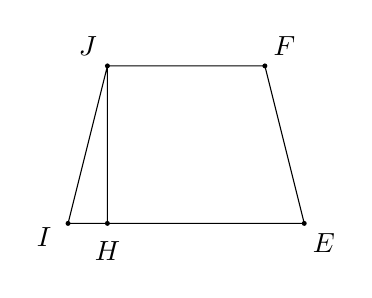
\begin{tikzpicture}[scale=.5]
						\coordinate (I)  at (0,0);
						\coordinate (H) at (1,0); 
						\coordinate  (E) at (6,0);
						\coordinate  (J) at (1,4);
						 \coordinate (F) at (5,4);
						\draw  (I)--(J)--(F)--(E)--(I)
						(J)--(H); 
						 \foreach \t/\g in {I/-150,E/-45,F/45,J/135,H/-90}{
						\fill (\t) circle (1.8pt) node[shift={(\g:10pt)}]{$ \t  $};}
					\end{tikzpicture}
			\end{minipage}
		\end{center}
		Ta có $\heva{&I \in (IJM) \cap (ABC)\\&AB \subset (ABC)\\&AB \parallel (IJM)}$ suy ra $(IJM) \cap (ABC) = IE  \parallel AB$ với $E \in BC \quad(1)$.\\
		Tương  tự $\heva{&J \in (IJM) \cap (ABD)\\&AB \subset (ABD)\\&AB \parallel (IJM)}$ suy ra $(IJM) \cap (ABD) = IF \parallel AB$ với $F \in BD \quad(2)$.\\
		Từ $(1)$ và $(2)$ ta được $(IJM) \cap (BCD) = EF$. Mà $M \in (IJM) \cap (BCD)$ suy ra  $M \in EF$.\\
		Do $IE$  và $JF$ cùng song song với $AB$ nên tứ diện $IEFJ$ là hình thang. \\
		Trong tam giác $ABC$, ta có $\dfrac{IE}{AB}=\dfrac{CI}{CA}=\dfrac{1}{2}$ suy ra  $IE=\dfrac{AB}{2}=\dfrac{3}{2}$.\\
		Trong tam  giác $ABD$, ta có $\dfrac{JF}{AB}=\dfrac{DJ}{DA}=\dfrac{1}{3}$ suy ra $JF=\dfrac{AB}{3}=1$. \\
		Áp dụng định lí hàm số côsintrong tam giác  $AIJ$, ta có
		 \[IJ=\sqrt{AI^2+AJ^2-2AI\cdot AJ\cos 60^{\circ}}=\dfrac{\sqrt{13}}{2}.\]
		Tương tự ta cũng có $EF=\dfrac{\sqrt{13}}{2}$. \\ 
		Trong hình  thang cân $IEFJ$. Hạ $JH$ vuông góc với $IE$, ta có \\
		\[JH=\sqrt{IJ^2-IH^2}=\sqrt{IJ^2-{\left(\dfrac{IE-JE}{2}\right)}^2}=\dfrac{a\sqrt{51}}{12}.\] 
		Vậy $S_{IEFJ}=\dfrac{1}{2}(IE+JF)\cdot JH=\dfrac{5\cdot  3^2\sqrt{51}}{144} \approx 2{,}23$.
	 }
\end{ex}

% nguồn: Ok_TraLoiNgan_Lop11_Lan2
\begin{ex}%[1H4V4-4]%[ma:fe19822e]
	Cho hình lập phương $ABCD.A'B'C'D'$ cạnh $a$. Xét tứ diện $AB'CD'$. Cắt  tứ diện đó bằng mặt phẳng đi qua tâm của hình lập phương và song song với mặt phẳng $\left(ABC\right)$. Tính diện tích của thiết diện thu được khi $a=6$.
	\begin{center}
		\begin{tikzpicture}[scale=1,font=\footnotesize,line join=round,line cap=round,>=stealth]
				\path (0,3) coordinate (h) 
					(0,0) coordinate (B)++(3,0) coordinate (C)++(0.8,1) coordinate  (D)
					($(B)+(D)-(C)$) coordinate (A); 
				\foreach \p  in {A,B,C,D}\path ($(\p)+(h)$) coordinate (\p');
				 \draw (A')--(B')--(B)--(C)--(D)--(D')--cycle (B')--(C')--(D')
					(C)--(B')--(D')--(C)--(C'); 
				 \draw[dashed] (B)--(A)--(D)
					(B')--(A)--(A') 
					 (D')--(A)--(C);
				 \foreach \p/\g in {A/150,B/240,C/-60,D/0,A'/90,B'/180,C'/-30,D'/45} \fill[black] (\p) circle (1pt)+(\g:0.3) node{$\p$};
			\end{tikzpicture}
	\end{center}
	\shortans{18} 
	\loigiai{ 
		\begin{center}
			\begin{tikzpicture}[scale=1,font=\footnotesize,line join=round,line cap=round,>=stealth]
					\path (0,3) coordinate (h) 
						(0,0)  coordinate (B)++(3,0) coordinate (C)++(0.8,1) coordinate (D)
						($(B)+(D)-(C)$) coordinate  (A);
					\foreach \p in {A,B,C,D}\path  ($(\p)+(h)$) coordinate (\p');
					\path ($(A)!0.5!(A')$)  coordinate (I)
						 ($(A)!0.5!(B')$) coordinate (J)
						($(C)!0.5!(B')$) coordinate  (K)
						 ($(C)!0.5!(D')$) coordinate (L)
						 ($(A)!0.5!(D')$) coordinate (M)
						($(C)!0.5!(A')$)  coordinate (O);
					 \draw[fill=pink,dashed] (M)--(J)--(K)--(L)--cycle;
					\draw (A')--(B')--(B)--(C)--(D)--(D')--cycle (B')--(C')--(D') 
						 (C)--(B')--(D')--(C)--(C');
					 \draw[dashed] (B)--(A)--(D)
						 (B')--(A)--(A')
						 (D')--(A)--(C)
						(O)--(I); 
					\foreach \p/\g in {A/150,B/240,C/-60,D/0,A'/90,B'/180,C'/-30,D'/45,O/0,I/45,J/-120,K/-120,L/-30,M/90} \fill[black] (\p) circle (1pt)+(\g:0.3)  node{$\p$};
				\end{tikzpicture}
		\end{center}
		Cách xác định mặt phẳng thiết diện tạo bởi mặt phẳng đi qua tâm của  hình lập phương và song song với mặt phẳng $\left(ABC\right)$với tứ diện $AB'CD'$ như sau.\\
		Trong $\left(ACC'A'\right)$ kẻ  đường thẳng qua $O$ và song song với $AC$, cắt $AA'$ tại trung điểm $I$.\\
		Trong $\left(ABB'A'\right)$ kẻ đường thẳng quan $I$ song song với $AB$, cắt $AB'$ tại trung điểm  $J$.\\
		Trong $\left(B'AC\right)$ kẻ đường thẳng qua $J$ song song với $AC$, cắt  $B'C$ tại trung điểm $K$.\\
		Trong $\left(B'CD'\right)$ kẻ đường thẳng qua $K$ song song với  $B'D'$, cắt $D'C$ tại trung điểm $L$.\\
		Trong $\left(D'AC\right)$ kẻ đường thẳng qua $L$ song song với $AC$, cắt $AD'$  tại trung điểm $M$.\\
		Mặt phẳng vừa tạo thành  song song với $\left(ABC\right)$ và tạo với tứ diện $AB'CD'$ thiết diện là hình bình hành $MJKL$.\\
		 Ta có
		$JM=\dfrac{1}{2}B'D'=\dfrac{1}{2}AC=ML$ nên tứ giác  $MJKL$ là hình thoi.\\
	Vậy diện tích của thiết diện là $$S_{MJKL}=\dfrac{1}{2}\cdot JL\cdot MK=\dfrac{1}{2}\cdot a\cdot a=\dfrac{a^2}{2}=\dfrac{6^2}{2}=18.$$} 
\end{ex}

% nguồn: Ok_TraLoiNgan_Lop11_Lan2
\begin{ex}%[1H4V4-4]%[ma:643a3721]
	Cho hình chóp $S.ABCD$ có đáy $ABCD$ là hình bình hành, mặt bên $SAB$ là tam giác vuông tại $A$, $SA=a\sqrt{3}$, $SB=2a$. Điểm  $M$ nằm trên đoạn $AD$ sao cho $AM=2MD$. Gọi $\left(P\right)$ là mặt phẳng qua $M$ và song song với $\left(SAB\right)$. Khi $a=7$, tính diện tích thiết diện của hình chóp cắt bởi mặt phẳng $\left(P\right)$.
	 \shortans{23,6}
	\loigiai{ 
		\begin{center}
			\begin{tikzpicture}[scale=1,font=\footnotesize,line join=round,line cap=round,>=stealth]
					 \path (0,0) coordinate (B)++(3,0) coordinate (C)++(1.5,1) coordinate (D)
						($(B)+(D)-(C)$) coordinate  (A)
						(-0.5,2.5)  coordinate (h)
						($(A)+(h)$) coordinate  (S)
						 ($(A)!2/3!(D)$) coordinate (M)
						($(B)!2/3!(C)$)  coordinate (N)
						 ($(S)!2/3!(D)$) coordinate (Q)
						($(S)!2/3!(C)$)  coordinate (P);
					\draw (S)--(B)--(C)--(D)--cycle  (S)--(C)
						 (N)--(P)--(Q);
					 \draw[dashed] (S)--(A)--(B)
						(A)--(D) 
						 (N)--(M)--(Q);
					\foreach \p/\g in {A/60,B/240,C/-60,D/0,S/90,M/-60,N/-90,P/60,Q/45} \fill[black] (\p) circle  (1pt)+(\g:0.3) node{$\p$};
					\foreach \x/\y/\z in {S/A/B,P/Q/M,Q/M/N} \draw pic[draw,angle radius=0.2cm]{right angle=\x--\y--\z}; 
				\end{tikzpicture}
		\end{center}
		Ta  có
		\begin{itemize}
			\item $\heva{&\left(P\right)\parallel \left(SAB\right) \\&M\in AD,M\in \left(P\right)}$ $\Rightarrow \heva{&\left(P\right)\cap \left(ABCD\right)=MN \\&\left(P\right)\cap  \left(SCD\right)=PQ}$ và $MN\parallel PQ\parallel AB$,
			\item 
			 $\heva{&\left(P\right)\parallel \left(SAB\right) \\&M\in AD,M\in \left(P\right)}$ $\Rightarrow \heva{&\left(P\right)\cap \left(SAD\right)=MQ \\&\left(P\right)\cap \left(SBC\right)=NP}$ và $\heva{&MQ\parallel SA \\&NP\parallel SB.}$
		\end{itemize}
		Mà tam giác $SAB$ vuông tại $A$ nên $SA\perp AB$ $\Rightarrow  MN\perp MQ$.\\
		Do đó, $\left(P\right)$ cắt hình chóp theo thiết diện là hình thang vuông  tại $M$ và $Q$.\\
		Mặt  khác
		$MQ\parallel SA$ $\Rightarrow \dfrac{MQ}{SA}=\dfrac{DM}{DA}=\dfrac{DQ}{DS}$  $\Rightarrow MQ=\dfrac{1}{3}SA$ và $\dfrac{DQ}{DS}=\dfrac{1}{3}$.\\
		Tương tự, $PQ\parallel CD$ $\Rightarrow \dfrac{PQ}{CD}=\dfrac{SQ}{SD}$ $\Rightarrow PQ=\dfrac{2}{3}AB$,  với $AB=\sqrt{SB^2-SA^2}=a$.\\
	Khi đó  $S_{MNPQ}=\dfrac{1}{2}MQ\cdot\left(PQ+MN\right)=\dfrac{1}{2}\dfrac{SA}{3}\cdot\left(\dfrac{2AB}{3}+AB\right)=\dfrac{5a^2\sqrt{3}}{18}=\dfrac{5\cdot 7^2\sqrt{3}}{18}\approx 23{,}6$.}
\end{ex}


%%%%%%%%%%%%%%%% TỰ LUẬN %%%%%%%%%%%%%%%%

% nguồn: Ok_TuanLuan_Toan11_Lan2
\begin{ex}%[1H4H4-4]%[ma:02cc6572]
	Cho hình hộp $ABC D.A'B'C'D'$. Gọi $M$ là trung điểm của $A'B'$. Tìm thiết diện của hình hộp cắt bởi mặt  phẳng $(P)$ đi qua $M$ và song song với mặt phẳng $(AA'C')$. Thiết diện là hình gì?
	 \loigiai{
	Vì $(P)$ song song với $(AA'C)$  nên $(P)$ song song với $(A'C'CA)$.\\
	Suy ra giao tuyến  của $(P)$ với $(A'B'C'D')$ là đường thẳng đi qua $M$, song song với $A'C'$ và cắt $B'C'$ tại trung diểm $N$ của $B'C'$.\\
	Tương tự, giao tuyến của $(P)$ với $(B'C'CB)$ là đường thẳng di qua $N$, song song với $C'C$ và cắt  $B C$ tại trung diểm $P$ của $BC$.
	\begin{center}
		\begin{tikzpicture}[scale=0.7,font=\footnotesize,line join=round,line cap=round,>=stealth]
				\coordinate (A) at (0,0); 
				 \coordinate (B) at (-2,-2);
				\coordinate  (C) at (4,-2);
				\coordinate (D) at (6,0); 
				\coordinate  (A') at ($(A)+(0,5)$);
				\coordinate (B') at ($(B)+(0,5)$); 
				\coordinate (C') at  ($(C)+(0,5)$);
				\coordinate (D') at ($(D)+(0,5)$); 
				\coordinate  (M) at ($(A')!0.5!(B')$);
				\coordinate (N) at  ($(B')!0.5!(C')$);
				 \coordinate (P) at ($(B)!0.5!(C)$);
				\coordinate (Q) at ($(A)!0.5!(B)$); 
				 \fill[yellow](M)--(N)--(P)--(Q)--cycle;
				\draw (B)--(C)--(C')--(B')--cycle (C)--(D)--(D')--(C') 
					 (C')--(A')--(B')--(B)
					(A')--(D') 
					 (M)--(N)--(P);
				 \draw[dashed](B)--(A)--(A')
					(D)--(A)--(C) 
					 (P)--(Q)--(M);
				\foreach \i/\g in  {A/-90,B/-90,C/-45,D/0,A'/90,B'/180,C'/90,D'/0,M/135,N/45,Q/180,P/-90}{\draw[fill](\i) circle (1pt)
					($(\i)+(\g:3mm)$)  node[scale=1]{$\i$};}
			\end{tikzpicture}
	\end{center}
	Giao tuyến của $(P)$ với $(A'B'BA)$ là đường  thẳng đi qua $M$, song song với $A'A$ và cắt $AB$ tại trung điểm $Q$ của $AB$.\\
	Vậy thiết diện cần  tìm là tứ giác $MNPQ$.\\
	Do $NP$ song song và bằng $CC'$; $MQ$ song  song và bằng $AA'$ nên tứ giác $MNPQ$ là hình bình hành.
	 }
\end{ex}

% nguồn: Ok_TuanLuan_Toan11_Lan2
\begin{ex}%[1H4H4-4]%[ma:b0b56751]
	Cho hình chóp $S.ABC$. Gọi $M$ là trung điểm $S A$. Xác định thiết diện của hình chóp cắt bởi mặt phẳng $(P)$ đi qua $M$ và song song với mặt phẳng $(ABC)$. 
	\loigiai{ 
	\begin{center}
		\begin{tikzpicture}[scale=0.7,font=\footnotesize,line join=round,line cap=round,>=stealth]
				\coordinate (S) at  (0,4);
				\coordinate  (A) at (-2,0);
				\coordinate (B) at (0,-3); 
				\coordinate (C)  at (3,0);
				\coordinate  (M) at ($(S)!0.5!(A)$);
				\coordinate (N) at  ($(S)!0.5!(B)$);
				\coordinate (P) at ($(S)!0.5!(C)$); 
				 \fill[yellow](M)--(N)--(P)--cycle;
				\draw (S)--(A) 
					(S)--(B) 
					 (S)--(C)
					(B)--(C) 
					(A)--(B) 
					 (M)--(N)--(P);
				\draw[dashed](A)--(C) 
					 (M)--(P);
				\foreach \i/\g in {S/90,A/180,B/-90,C/0,M/180,N/-45,P/0}{\draw[fill](\i) circle  (1pt)
					($(\i)+(\g:3mm)$)  node[scale=1]{$\i$};}
			\end{tikzpicture}
	\end{center}
	Ta có $M$ là một điểm chung  của $(P)$ và $(SAB)$.\\
	Do $\heva{&(P)\parallel(ABC)\\&(SAB)\cap(ABC)=AB}$ nên giao tuyến của $(P)$  và $(SAB)$ là đường thẳng đi qua $M$ song song với $A B$ và cắt $S B$ tại trung điểm $N$ của $SB$.\\
	Tương tự, giao tuyến của $(P)$ và $(SAC)$ là đường thẳng đi qua $M$, song song với $AC$ và cắt $S C$ tại  trung điểm $P$ của $SC$.\\
	Vậy thiết  diện của hình chóp $S.ABC$ cắt bởi mặt phẳng $(P)$ là tam giác $MNP$.
	} 
\end{ex}

% nguồn: Ok_TuanLuan_Toan11_Lan2
\begin{ex}%[1H4H4-4]%[ma:7e191b69]
	Cho hình hộp $ABCD.A'B'C'D'$. Gọi $K$  là trung điểm $C D$. Gọi $(P)$ là mặt phẳng đi qua $C'$ và song song với $\left(A'A K\right)$. Xác định thiết diện của hình hộp cắt bởi mặt phẳng $(P)$.
	\loigiai{\begin{center}
	\begin{tikzpicture}[scale=0.8,font=\footnotesize,line join=round,line cap=round,>=stealth]
			\coordinate (A)  at (0,0);
			\coordinate  (B) at (-2,-2);
			\coordinate (C)  at (4,-2);
			\coordinate  (D) at (6,0);
			\coordinate (A')  at ($(A)+(0,5)$);
			 \coordinate (B') at ($(B)+(0,5)$);
			\coordinate (C') at  ($(C)+(0,5)$);
			\coordinate (D')  at ($(D)+(0,5)$);
			\coordinate (H) at ($(C')!0.5!(D')$); 
			 \coordinate (K) at ($(C)!0.5!(D)$);
			\coordinate (M) at  ($(A')!0.5!(B')$);
			\coordinate (N) at ($(A)!0.5!(B)$); 
			 \fill[yellow](M)--(C')--(C)--(N)--cycle;
			\draw (B)--(C)--(C')--(B')--cycle  (C)--(D)--(D')--(C')
				 (C')--(A')--(B')--(B)
				 (A')--(D')
				 (A')--(H)--(K)
				(M)--(C'); 
			\draw[dashed]  (M)--(N)--(C)
				(A')--(K)--(A)--cycle  (B)--(A)--(D);
			\foreach \i/\g  in {A/-90,B/-90,C/-45,D/0,A'/90,B'/180,C'/90,D'/0,M/135,N/180,K/-45,H/90}{\draw[fill](\i) circle (1pt)
				($(\i)+(\g:3mm)$)  node[scale=1]{$\i$};}
		\end{tikzpicture}
\end{center}
Gọi $H$ là trung điểm $C'D'$.\\ 
$\Rightarrow K H \parallel AA'$ $\Rightarrow H \in\left(A'A  K\right)$.\\
Qua $C'$  kẻ đường thẳng song song với $A'H$, cắt $A'B'$ tại $M$.\\
Qua $C$ kẻ đường thẳng  song song với $A K$, cắt $A B$ tại $N$.\\
Suy ra mặt phẳng $(CC'MN)$ là mặt phẳng đi qua $C'$ và song song với  $\left(A'A K\right)$.\\
Thiết diện  cần tìm là hình bình hành $CC'MN$.
 }
\end{ex}

% nguồn: Ok_TuanLuan_Toan11_Lan2
\begin{ex}%[1H4H4-4]%[ma:234a46dd]
	Cho hai hình bình hành $ABCD$  và $ABEF$ không cùng nằm trong một mặt phẳng.
	\begin{enumerate}
		\item Chứng minh rằng  $\left(AFD\right)\parallel\left(BEC\right)$.
		\item Gọi $M$ là trọng tâm của tam  giác $ABE$. Gọi $(P)$ là mặt phẳng đi qua $M$ và song song với mặt phẳng $\left(AFD\right)$. Lấy $N$ là giao điểm của $(P)$ và $AC$. Tính $\dfrac{AN}{NC}$.
	\end{enumerate}
	\loigiai{ 
		\begin{center}
			\begin{tikzpicture}[scale=1,font=\footnotesize,line join=round,line cap=round,>=stealth]
					 \path
						(0,0) coordinate  (A)
						(-2,-1) coordinate (D) 
						 (4,0) coordinate (B)
						($(D)+(B)-(A)$) coordinate  (C)
						(A)+(1,2)  coordinate (F)
						 ($(F)+(B)-(A)$) coordinate (E)
						 ($(F)!.5!(B)$) coordinate (O)
						($(O)!1/3!(B)$) coordinate  (M)
						($(B)!1/3!(A)$) coordinate (H) 
						($(C)!1/3!(A)$) coordinate  (N);
					 \draw (D)--(C)--(B)--(E)--(F)--cycle (C)--(E);
					\draw[dashed]  (D)--(A)--(B)--(F)--(A)--(C)
						(N)--(H)--(M) 
						(A)--(E); 
					\foreach \p/\r  in {A/180,D/180,C/-60,B/0,N/-130,H/120,M/90,O/90,F/90,E/90}
					\fill (\p)  circle (1pt) node[shift={(\r:3mm)}]{$\p$};
				\end{tikzpicture}
		\end{center}
		\begin{enumerate}
			\item Ta có $AD\parallel BC$, $AD\not\subset(BCE)$ và $BC\subset(BCE)$, suy ra $AD\parallel\left(BCE\right)$.  \\
			Tương tự  $AF\parallel \left(BCE\right)$.\\
			Mà  $AF$ cắt $AD$ tại $A$.\\
			Suy  ra $\left(ADF\right)\parallel\left(BCE\right)$.
			\item Ta có $(P)\parallel\left(AFD\right)$ nên  $(P)\cap\left(ABF\right)=MH$ với $M\in $ $FB$ và $MH\parallel AF$.\\
			Vì $M$ là trọng tâm của tam giác $ABE$ nên $\dfrac{BM}{BO}=\dfrac{2}{3}$ với $O$ là tâm  hình bình hành $ABEF$.\\
			Vì $ABEF$ là hình  bình hành nên $\dfrac{\dot{B}O}{BF}=\dfrac{1}{2}$. \\
			Suy  ra $\dfrac{BM}{BF}=\dfrac{1}{3}$. Do đó $\dfrac{BM}{MF}=\dfrac{1}{2}$.\\
			Khi đó $\dfrac{BH}{AH}=\dfrac{1}{2}$ (vì  $AF\parallel MH$) mà $(P)\parallel\left(AFD\right)$ nên $(P)\cap\left(ABC\right)=NH$ với $N\in AC$ và$NH\parallel AD$.\\
			Do đó $\dfrac{AN}{NC}=\dfrac{AH}{BH}=2$. 
		\end{enumerate}
	} 
\end{ex}

% nguồn: Ok_TuanLuan_Toan11_Lan2
\begin{ex}%[1H4H4-4]%[ma:93eb1a78]
	Cho hình chóp $S.ABCD$ có đáy $ABCD$ là  hình bình hành và $M$ là trung điểm của $AB$. Xác định thiết diện của hình chóp cắt bởi $(\alpha)$ đi qua $M$ và song song với mặt phẳng $(SAD)$.Thiết diện là hình gì?
	 \loigiai{
		\begin{center}
			\begin{tikzpicture}[scale=1.5,font=\footnotesize,line join=round,line cap=round,>=stealth]
					 \def\a{3}
					 \def\b{1.5}
					\def\g{30} 
					\def\h{2} 
					 \path
						(0:0) coordinate (A)--++(\g:\b) coordinate (B)--++(0:\a) coordinate (C)--++(\g-180:\b) coordinate  (D)
						(A)--++(70:3.5)  coordinate (S);
					\draw ($(A)!.5!(B)$)  coordinate (M);
					\draw  ($(C)!.5!(D)$) coordinate (N);
					\draw  ($(S)!.5!(B)$) coordinate (K);
					\draw  ($(S)!.5!(C)$) coordinate (H);
					\foreach \x/\g in  {A/180,B/150,C/0,D/-30,S/90,M/160,N/-60,K/-50,H/40}
					\fill(\x) circle (1pt) 
						($(\x)+(\g:3mm)$) node{$\x$}; 
					 \draw[dashed] (S)--(B)--(A)
						 (C)--(B)
						 (N)--(M)--(K)--(H);
					\draw (S)--(A)--(D)--(C)--(S)--(D) 
						 (H)--(N);
				\end{tikzpicture}
		\end{center}
		Ta có $(\alpha)\parallel (SAD) \Rightarrow\heva{&(\alpha) \parallel  SA \\ &(\alpha) \parallel SD \\& (\alpha) \parallel AD.}$\\
		Ta có $\heva{&M \in (SAB) \cap (\alpha) \\ & (SAB) \supset SA \\ &(\alpha) \parallel SA} \Rightarrow (SAB) \cap(\alpha)=MK \parallel SA,  K \in S B$.\\
		Ta có $\heva{&M \in(ABCD) \cap (\alpha) \\& (ABCD) \supset AD \parallel (\alpha) \parallel AD} \Rightarrow (ABCD) \cap (\alpha)=MN \parallel AD, N \in CD$.\tagEX{1} 
		\noindent Tương tự $\heva{&N \in (SCD) \cap (\alpha) \\ &(\alpha) \parallel SD \parallel (SCD) \supset SD} \Rightarrow (SCD) \cap (\alpha)=NH  \parallel SD, H \in SC$.\\
		Dễ thấy $HK=(\alpha) \cap (SBC), HK \parallel AD$  do $(\alpha) \parallel AD \parallel BC$.\tagEX{2}
		\noindent Từ (1) và (2) suy  ra $MN \parallel HK$.\\
		Thiết diện  là hình thang $MNHK$ ($MN\parallel HK$).
	} 
\end{ex}

% nguồn: Ok_TuanLuan_Toan11_Lan2
\begin{ex}%[1H4V4-4]%[ma:9aa1ba68]
	Cho hình chóp $S.ABCD$ có đáy là  hình thoi cạnh $a$, tam giác $SAD$ là tam giác đều. Gọi $M$ là một điểm thuộc cạnh $A B, A M=x$ với $0<x<a$. Mặt phẳng $(P)$ đi qua $M$ song song với $(SAD)$. Tính diện tích thiết diện của hình chóp $S.ABCD$ cắt bởi mặt phẳng $(P)$.
	 \loigiai{
	\begin{center}
		\begin{tikzpicture}[scale=1,font=\footnotesize,line join=round,line cap=round,>=stealth]
				\coordinate (A)  at (0,0);
				\coordinate (B) at (-2,-3); 
				\coordinate (D) at (7,0); 
				\coordinate (C) at ($(B)+(D)-(A)$); 
				\coordinate (S)  at ($(A)+(1,5)$);
				\coordinate (M)  at ($(A)!0.5!(B)$);
				\coordinate  (N) at ($(C)!0.5!(D)$);
				 \coordinate (F) at ($(S)!0.5!(C)$);
				\coordinate (E) at ($(S)!0.5!(B)$); 
				 \coordinate (H) at ($(N)!0.42!(M)$);
				\fill[yellow](M)--(N)--(F)--(E)--cycle; 
				 \draw (S)--(B)
					(S)--(C) 
					 (S)--(D)
					 (B)--(C)--(D)
					(F)--(N) 
					(F)--(E); 
				\draw[dashed](S)--(A) 
					(A)--(B) 
					 (A)--(D)
					 (A)--(C)
					(B)--(D) 
					 (N)--(M)--(E)
					 (F)--(H);
				\foreach  \i/\g in {S/90,A/-90,B/-90,C/-90,D/0,N/0,H/-45,M/-90,E/135,F/45}{\draw[fill](\i) circle (1pt)
					($(\i)+(\g:3mm)$)  node[scale=1]{$\i$};}
			\end{tikzpicture}
	\end{center}
	Do mặt phẳng $(P)$ đi qua điểm $M$  và song song với $(SAD)$ nên cắt các cạnh của hình chóp bằng các giao tuyến đi qua $M$ và song song với mặt phẳng $(SAD)$.\\
	Do $ABCD$ là hình thoi  và tam giác $SAD$ dều nên thiết diện thu được là hình thang cân $MNFE$ với $MN \parallel EF$, $M E=NF$.\\
	Khi đó $MN=a$, $\dfrac{E  F}{B C}=\dfrac{SF}{SC}=\dfrac{M A}{A B}=\dfrac{x}{a}$\\
	 $\Rightarrow EF=x$ và $MF=a-x$.\\
	 Kẻ đường cao $FH$, $H \in M N$ ta có \[FH=\sqrt{MF^2-\left(\dfrac{MN-EF}{2}\right)^{2}}=\dfrac{\sqrt{3}}{2}(a-x).\]
	Vậy diện tích hình thang là  \[S=\dfrac{\sqrt{3}}{4}\left(a^{2}-x^{2}\right).\]
	} 
\end{ex}

% nguồn: Ok_TuanLuan_Toan11_Lan2
\begin{ex}%[1H4V4-4]%[ma:dffd2d30]
	Cho hình chóp $S. A B C D$ có  đáy là hình thang $A B C D$ có $A D\parallel B C$,\\ $AD=2BC$. Gọi $E$ là trung điểm $AD$ và $O$ giao điểm của $A C$ và $BE$; $I$ là một điểm di động trên đoạn $A C$ khác $A$ và $C$. Qua $I$ vẽ mặt phẳng $(\alpha)$ song song với $(SBE)$. Tìm thiết diện tạo bởi $(\alpha)$ và hình chóp $S .ABCD$.
	 \loigiai{
	\begin{center}
		\begin{tikzpicture}[scale=1,font=\footnotesize,line join=round,line cap=round,>=stealth]
				\coordinate (S) at (1.5,4); 
				\coordinate (A)  at (0,0);
				\coordinate (B) at  (1,-2);
				\coordinate (C) at  (4,-2);
				 \coordinate (D) at (6,0);
				\coordinate (M) at  ($(A)!0.5!(B)$);
				\coordinate (E) at  ($(A)!0.5!(D)$);
				\coordinate (H)  at ($(B)!0.5!(C)$);
				\coordinate  (K) at ($(S)!0.5!(C)$);
				\coordinate  (P) at ($(S)!0.5!(A)$);
				 \coordinate (V) at ($(S)!0.5!(D)$);
				\coordinate  (N) at ($(A)!0.5!(E)$);
				\coordinate (U)  at ($(D)!0.5!(E)$);
				\coordinate (O)  at ($(A)!0.5!(C)$);
				 \coordinate (I) at ($(A)!0.5!(O)$);
				 \fill[yellow](M)--(N)--(P)--cycle (K)--(V)--(U)--(H)--cycle;
				 \draw (S)--(A)
					(S)--(B) 
					(S)--(C) 
					(S)--(D) 
					(B)--(C) 
					(A)--(B)--(C)--(D) 
					 (P)--(M)
					(V)--(K)--(H); 
				\draw[dashed](A)--(D) 
					 (V)--(U)--(H)
					 (M)--(N)--(P)
					(A)--(C) 
					(B)--(E)--(S); 
				\foreach  \i/\g in {S/90,A/180,B/-90,C/-90,D/0,M/200,P/180,N/-45,O/-90,H/-90,U/-45,V/45,I/-90,E/-90,K/80}{\draw[fill](\i) circle (1pt)
					($(\i)+(\g:3mm)$) node[scale=1]{$\i$};} 
			\end{tikzpicture}
	\end{center}
	\begin{itemize}
		\item \textbf{Trường hợp 1:}  Điểm $I$ nằm giữa $A$ và $O$.\\
		Qua $I$ kẻ đường  thẳng song song với $B E$ cắt $A B, A D$ lần lượt tại $M$ và $N$.\\
		Qua $M$ kẻ đường thẳng song song với $S B$ cắt  $S A$ tại $P$.\\
		Suy ra $(MNP)$ là mặt phẳng đi qua $I$ và song song với  $(SBE)$.\\
		Do đó, thiết diện của hình chóp cắt bởi mặt  phẳng ( $\alpha$) là tam giác $M N P$.
		\item \textbf{Trường hợp 2:} Điểm $I$ nằm  giữa $C$ và $O$.\\
		Qua $I$ kẻ đường thẳng song song với $B E$  cắt $BC$, $AD$ lần lượt tại $H$ và $U$.\\
		Qua $H$  kẻ đường thẳng song song với $S B$ cắt $SC$ tại $K$.\\
		 Qua $U$ kẻ đường thẳng song song với $S E$ cắt $SD$ tại $V$.\\
		Suy ra $(HKVU)$ là mặt phẳng đi qua $I$ và  song song với $(SBE)$.\\
		Do đó thiết diện của hình  chóp cắt bởi mặt phẳng $(\alpha)$ là tứ giác $(HKVU)$.
	\end{itemize}
	 }
\end{ex}

% nguồn: Ok_TuanLuan_Toan11_Lan2
\begin{ex}%[1H4V4-4]%[ma:071504be]
	Cho hình chóp $S.ABCD$ có đáy $ABCD$ là hình vuông cạnh bằng $a$, tam giác $SAB$ đều, $SC=SD=a\sqrt{3}$. Gọi $H$, $K$ lần lượt là trung điểm của $SA$, $SB$ và $M$ là một điểm trên cạnh $AD$, mặt phẳng $(HKM)$ cắt $BC$ tại $N$. Đặt $AM=x\,(0\leq x \leq a)$. Tính giá trị $x$ để diện tích thiết diện $HKMN$ đạt giá trị  nhỏ nhất.
	 \loigiai{
		\begin{center}
			\begin{tikzpicture}[scale=1.5,font=\footnotesize,line join=round,line cap=round,>=stealth]
					 \def\a{3}
					\def\b{1.5} 
					\def\g{30} 
					\def\h{2} 
					 \path
						(0:0) coordinate (A)--++(\g:\b) coordinate (B)--++(0:\a) coordinate (C)--++(\g-180:\b)  coordinate (D)
						 (A)--++(70:3.5) coordinate (S);
					\draw ($(A)!.5!(D)$)  coordinate (M);
					\draw  ($(C)!.5!(B)$) coordinate (N);
					\draw  ($(S)!.5!(B)$) coordinate (K);
					\draw ($(S)!.5!(A)$) coordinate (H); 
					\foreach \x/\g in {A/180,B/60,C/0,D/-30,S/90,M/-90,N/60,K/50,H/180} 
					 \fill(\x) circle (1pt)
						($(\x)+(\g:3mm)$)  node{$\x$};
					\draw[dashed]  (S)--(B)--(A)
						 (C)--(B)
						 (M)--(N)--(K)--(H);
					 \draw (S)--(A)--(D)--(C)--(S)--(D)
						(H)--(M); 
				\end{tikzpicture}
		\end{center}
		Mặt phẳng $(HKM)$ và $(ABCD)$ chứa hai đường thẳng song song $HK$ và $AB$ nên giao tuyến của  chúng là $MN$ cũng song song với $HK$ và $AB$.\\
		Xét hai  tam giác $HAM$ và $KBN$ ta có
		 $BN=AM$, $BK=AH$, $\widehat{KBN}=\widehat{MHA}$ nên $\triangle HAM=\triangle KBN$.
		Từ đó  suy ra $MH=KN$.\\
		Vậy $MHKN$ là  hình thang cân có hai đáy $MN=a$, $HK=\dfrac{a}{2}$.\\
		Sử  dụng Định lý
		Cosin cho tam giác $SAD$ với $\cos \widehat{HAD}=-\dfrac{1}{2}$, ta  tính được
		 \[
		HM^2=HA^2+AM^2-2 HA \cdot AM \cdot\left(-\dfrac{1}{2}\right)=\dfrac{a^2+4x^2+2ax}{4}. 
		 \]
		 Đường cao của hình thang cân được tính bằng công thức
		 \[\sqrt{HM^2-\left(\dfrac{MN-HK}{2}\right)^2}=\dfrac{1}{2} \sqrt{16x^2+8ax+3a^2}.\]
		Do hai đáy có độ dài  không đổi nên diện tích thiết diện bé nhất khi đường cao bé nhất đạt khi $x=0$.
	 }
\end{ex}

% nguồn: Ok_TuanLuan_Toan11_Lan2
\begin{ex}%[1H4V4-4]%[ma:f28adced]
	Cho hình chóp $S.ABCD$ có đáy $ABCD$ là hình thang có $AD\parallel BC$, $AD=2BC$. Gọi $E$ là trung điểm của $AD$, $O$ là giao điểm của $AC$ và $BE$, $I$ là điểm nằm trên đoạn $OC$. Mặt phẳng $(P)$ qua $I$ và song song với $(SBE)$. Tìm các giao tuyến của các mặt  của hình chóp với mặt phẳng $(P)$.
	 \loigiai{
		\begin{center}
			\begin{tikzpicture}[scale=1,font=\footnotesize,line join=round,line cap=round,>=stealth]
					 \def\a{3}
					 \def\b{1}
					\def\g{30} 
					\def\h{2} 
					\path 
						 (0:0) coordinate (A)--++(0:3) coordinate (E)--++(0:3) coordinate (D)--++(-130:\a) coordinate (C)--++(180:3) coordinate (B)--++(70:7) coordinate (S);
					\draw[name  path=ac,dashed] (A)--(C);
					 \draw[name path=be,dashed] (B)--(E);
					\path[name  intersections={of=ac
						and  be}]
						(intersection-1)  coordinate (O);
					 \draw ($(A)!.7!(C)$) coordinate (I);
					\coordinate (X)  at ($(B)+(I)-(O)$);
					\coordinate (Y)  at ($(X)!3!(I)$);
					\path[name path=xy,dashed]  (X)--(Y);
					\path[name path=bc,dashed] (B)--(C); 
					\path[name path=ad,dashed] (A)--(D); 
					\path[name  intersections={of=xy
						 and ad}]
						(intersection-1) coordinate (N); 
					\path[name intersections={of=xy 
						and bc}] 
						 (intersection-1) coordinate (M);
					\coordinate  (Z) at ($(S)+(N)-(E)$);
					 \path[name path=sd,dashed] (S)--(D);
					 \path[name path=nz,dashed] (N)--(Z);
					\path[name  intersections={of=sd
						 and nz}]
						(intersection-1)  coordinate (P);
					 \path[name intersections={of=xy
						and  bc}]
						 (intersection-1) coordinate (M);
					 \coordinate (Z) at ($(S)+(N)-(E)$);
					\path[name path=sd,dashed]  (S)--(D);
					 \path[name path=nz,dashed] (N)--(Z);
					\path[name intersections={of=sd 
						and nz}] 
						(intersection-1) coordinate (P); 
					\coordinate  (T) at ($(M)+(P)-(N)$);
					 \path[name path=sc,dashed] (S)--(C);
					\path[name  path=pt,dashed] (P)--(T);
					\path[name  intersections={of=sc
						and  pt}]
						 (intersection-1) coordinate (Q);
					\foreach \x/\g  in {A/180,B/150,C/0,D/-30,S/180,E/90,O/-90,I/-90,M/-90,N/-60,P/0,Q/-30}
					\fill(\x) circle (1pt) 
						($(\x)+(\g:3mm)$) node{$\x$}; 
					\draw[dashed]  (A)--(D)
						(M)--(Y) 
						 (N)--(P);
					 \draw
						 (A)--(B)--(C)--(D)--(S)--(A)
						 (S)--(C)
						(S)--(D) 
						(S)--(B) 
						(Q)--(M)--(X) node[left]{$d$} 
						 (P)--(Z) node[right]{$x$}
						 (P)--(T) node[above]{$y$};
				\end{tikzpicture}
		\end{center}
		Ta có $(P)\parallel (SBE)$, $(ABCD) \cap(SBE)=BE$.\\ 
		Mà $I \in (P) \cap(ABCD)$  nên $(P) \cap(ABCD)= d$ với $d \parallel BE$.\\
		Trong mặt phẳng $(ABCD)$, gọi $M$ là giao điểm của $d$ và $BC$, $N$ là  giao điểm của $d$ và $AD$.\\
		Lúc đó $(P) \cap (ABCD)=MN$.\\ 
		Ta có $(P)\parallel (SBE)$, $(SBE) \cap (SAD)=SE$. Mà $N\in  (P) \cap(SAD)$ nên $(P)\cap(SAD)=Nx$ với $Nx \parallel SE$.\\
		Trong mặt phẳng $(SAD)$, gọi $P$ là giao điểm của $Nx$ và $SD$. Suy ra  $(P) \cap(SAD)=NP$.\\
		Ta có $MN \subset (P)$,  $CD\subset(SCD)$, $P\in (P)\cap(SCD)$, $MN \parallel CD$.\\
		Suy ra $(P)  \cap(SCD)=Py$ với $Py \parallel MN \parallel CD$.\\
		Trong mặt phẳng $(SCD)$, gọi $Q$ là giao điểm của $Py$ và  $SC$. Suy ra $(P)\cap(SCD)=PQ$.\\
		Ta có $Q \in SC$, suy ra $Q \in(SCB)$. Mà $Q \in(P)$, suy ra $Q  \in(SCB) \cap(P)$.\\
		Tương tự, ta có $M  \in (SCB) \cap(P)$. Suy ra $(P) \cap(SBC)=QM$.\\
	} 
\end{ex}

% nguồn: Ok_TuanLuan_Toan11_Lan2
\begin{ex}%[1H4V4-4]%[ma:88261ed6]
	Cho hình chóp $S.ABCD$ với $ABCD$ là hình thoi cạnh $a$, $SAD$ là tam giác đều. Gọi $M$ là một điểm thuộc cạnh $AB$, $AM=x$, $(P)$ là mặt phẳng qua $M$ song song với $(SAD)$. Tính diện tích thiết diện của hình chóp cắt bởi mặt  phẳng $(P)$.
	\loigiai{ 
		\begin{center}
			\begin{tikzpicture}[scale=1.5,font=\footnotesize,line join=round,line cap=round,>=stealth]
					\def\a{3} 
					\def\b{1.5} 
					 \def\g{30}
					 \def\h{2}
					 \path
						(0:0) coordinate (A)--++(\g:\b) coordinate (B)--++(0:\a) coordinate (C)--++(\g-180:\b)  coordinate (D)
						(A)--++(70:3.5) coordinate (S); 
					 \draw ($(A)!.5!(B)$) coordinate (M);
					\draw ($(C)!.5!(D)$) coordinate  (N);
					 \draw ($(S)!.5!(B)$) coordinate (F);
					\draw  ($(S)!.5!(C)$) coordinate (E);
					\foreach  \x/\g in {A/180,B/150,C/0,D/-30,S/90,M/160,N/-60,F/-50,E/40}
					 \fill(\x) circle (1pt)
						($(\x)+(\g:3mm)$) node{$\x$}; 
					\draw[dashed] (S)--(B)--(A) 
						 (C)--(B)
						 (N)--(M)--(F)--(E);
					\draw (S)--(A)--(D)--(C)--(S)--(D) 
						 (E)--(N);
				\end{tikzpicture}
		\end{center}
		 Do mặt phẳng $(P)$ đi qua $M$ và song song với $(SAD)$ nên cắt các mặt của hình chóp bằng các giao tuyến đi qua $M$ và song song với $(SAD)$. Do $ABCD$ là hình thoi và tam giác $SAD$ đều. Do đó thiết diện thu được là hình thang cân $MNEF$ ($MN \parallel EF$, $MF=EN$).\\
		 Khi đó ta có
		 $$
		MN=a,  \dfrac{EF}{BC}=\dfrac{SF}{SB}=\dfrac{MA}{AB}=\dfrac{x}{a} \Rightarrow EF=x; MF=a-x.
		$$ 
		Đường cao $FH$ của  hình thang cân bằng $FH=\sqrt{MF^2-\left(\dfrac{MN-EF}{2}\right)^2}=\dfrac{\sqrt{3}}{2}(a-x)$.\\
		Khi đó diện tích hình thang cân  là $S=\dfrac{\sqrt{3}}{4}\left(a^2-x^2\right)$.
	 }
\end{ex}

% nguồn: Ok_TuanLuan_Toan11_Lan2
\begin{ex}%[1H4V4-4]%[ma:d7ee613a]
	Cho hình chóp $S.ABCD$ có đáy là hình thang, đáy lớn $A D=3 a$,\\ $A B=B C=a$. Mặt bên $(SAD)$ là tam giác cân đỉnh $S$ với $SA=2a$, gọi $M$ là điểm thuộc cạnh $AB$ và không trùng với $A$, $B$. Mặt phẳng $(\alpha)$ đi qua $M$ và song song với $(SAD)$. Xác định thiết diện của chóp với  mặt phẳng $(\alpha)$. Thiết diện là hình gì?
	\loigiai{ 
	\begin{center}
		\begin{tikzpicture}[scale=0.9,font=\footnotesize,line join=round,line cap=round,>=stealth]
				\coordinate (S) at  (1,4);
				\coordinate (A) at  (0,0);
				 \coordinate (B) at (1,-2);
				\coordinate  (C) at (3,-2);
				 \coordinate (D) at (5,0);
				\coordinate (M)  at ($(A)!0.6!(B)$);
				\coordinate (N) at ($(D)!0.6!(C)$); 
				\coordinate (P) at  ($(S)!0.6!(C)$);
				\coordinate (Q) at ($(S)!0.6!(B)$); 
				\fill[yellow](M)--(N)--(P)--(Q)--cycle; 
				\draw  (S)--(A)
					(S)--(B) 
					 (S)--(C)
					 (S)--(D)
					 (B)--(C)
					 (A)--(B)--(C)--(D)
					(M)--(Q)--(P)--(N); 
				 \draw[dashed](A)--(D)
					 (M)--(N);
				\foreach \i/\g in {S/90,A/180,B/-90,C/-90,D/0,M/180,Q/180,P/45,N/0}{\draw[fill](\i) circle  (1pt)
					($(\i)+(\g:3mm)$)  node[scale=1]{$\i$};}
			\end{tikzpicture}
	\end{center}
	Qua $M$ kẻ đường thẳng  song song với $AD$, cắt $CD$ tại $N$.\\
	Qua $M$  kẻ đường thẳng song song với $SA$, cắt $SB$ tại $Q$.\\
	Qua $Q$ kẻ đường thẳng song song với $BC$, cắt $SC$ tại $P$.\\ 
	Suy ra $(MNPQ)$ là mặt phẳng qua $M$ và song  song với $(SAD)$.\\
	Do đó, thiết diện  của hình chóp $S.ABCD$ cắt bởi mặt phẳng $(P)$ là tứ giác $MNPQ$.\\
	Bởi vì $MN$ và $PQ$ cùng song song với $BC$ (hoặc $AD$) nên tứ giác $MNPQ$ là  hình thang.\\
	Áp dụng định lí Thales trong các tam giác $SAB$, $SBC$, $SCD$ ta được 
	\[\dfrac{BM}{BA}=\dfrac{M Q}{S A}=\dfrac{B Q}{B S}=\dfrac{CP}{CS}=\dfrac{C N}{C D}=\dfrac{N P}{S D} \Rightarrow \dfrac{M Q}{S A}=\dfrac{N P}{S D}.\] Mà tam giác $SAD$ cân  tại $S$ do đó $MQ=NP$.\\
	Vậy  $MNPQ$ là hình thang cân.
	 }
\end{ex}

% nguồn: Ok_TuanLuan_Toan11_Lan2
\begin{ex}%[1H4C4-4]%[ma:886ac390]
	Cho hình chóp $S.ABCD$ đáy là hình bình hành tâm $O$ có $A C=a$, $BD=b$. Tam giác $SBD$ là tam giác đều. Một mặt phẳng $(\alpha)$ di động song song với mặt phẳng $(SBD)$ và đi qua điểm $I$ trên đoạn $AC$ và không trùng với  $ A $, $ C $.
	\begin{enumerate}
		\item Xác định thiết diện  của hình chóp với mặt phẳng ( $\alpha$).
		\item Tính diện tích thiết diện theo  $a$, $b$ và $x=AI$.
	\end{enumerate}
	 \loigiai{
	\begin{center}
		\begin{tikzpicture}[scale=0.8,font=\footnotesize,line join=round,line cap=round,>=stealth]
				\coordinate (A) at  (0,0);
				\coordinate (B)  at (-2,-3);
				\coordinate (D) at (7,0); 
				 \coordinate (C) at ($(B)+(D)-(A)$);
				\coordinate  (S) at ($(A)+(1,5)$);
				 \coordinate (O) at ($(A)!0.5!(C)$);
				\coordinate (M) at  ($(A)!0.3!(D)$);
				\coordinate  (I) at ($(A)!0.3!(O)$);
				\coordinate (P)  at ($(A)!0.3!(S)$);
				\coordinate (N)  at ($(A)!0.3!(B)$);
				 \coordinate (L) at ($(B)!0.5!(C)$);
				\coordinate (H) at ($(D)!0.5!(C)$); 
				 \coordinate (K) at ($(S)!0.5!(C)$);
				\fill[yellow](M)--(N)--(P)--cycle (H)--(L)--(K)--cycle; 
				 \draw (S)--(B)
					(S)--(C) 
					 (S)--(D)
					(B)--(C)--(D) 
					 (K)--(L);
				\draw[dashed](S)--(A) 
					 (A)--(B)
					(A)--(D) 
					 (A)--(C)
					(B)--(D) 
					(N)--(M)--(P) 
					 (L)--(H)--(K)
					 (S)--(O)
					 (P)--(N);
				 \foreach \i/\g in {S/90,A/-90,B/-90,C/-90,D/0,N/180,M/-90,P/45,K/45,H/-90,L/-90,O/-90,I/-90}{\draw[fill](\i) circle (1pt)
					($(\i)+(\g:3mm)$) node[scale=1]{$\i$};} 
			\end{tikzpicture}
	\end{center}
	\begin{enumerate}
		\item 
		\begin{itemize}
			\item Nếu $I  $ nằm trên đoạn $ OA $ và $ I $ không trùng $ O $ và $ A $ thì ta có $\heva{&(\alpha)\parallel(P)\\&(ABD)\parallel(SBD)\\&I\in(\alpha)\cap(SBD).}$ \\
			Suy ra $(\alpha)  \cap(ABD)=MN$ với $MN$ qua $I$ và $MN\parallel BD$.\\
			Do đó theo Ta-lét,  ta có $ \dfrac{AN}{AB}=\dfrac{AM}{AD}=\dfrac{MN}{BD} \qquad (1).$\\
			Tương tự $(\alpha)$ cắt $(SAB)$ theo đoạn giao tuyến $M P$ song song với  $SB$ cắt $(SAD)$ theo đoạn giao tuyến $N P\parallel SD$.\\
			Do đó theo  Ta-lét, ta có $ \dfrac{AN}{AB}=\dfrac{AP}{AS}=\dfrac{NP}{SB} \qquad (2).$\\
			 Từ $ (1) $ và $ (2) $, ta có
			$$ \dfrac{AM}{AD} = \dfrac{AP}{AS} \Rightarrow MP  \parallel SD \Rightarrow \dfrac{AM}{AD} =\dfrac{MP}{SD} \qquad (3).$$
			Vậy $ (1) $, $ (2) $ và $ (3) $ suy ra $ \dfrac{MN}{BD}=\dfrac{NP}{SB}=\dfrac{MP}{SD}$,  kết hợp với $ SB=BD=SD $ nên $ \triangle MNP $ là tam giác đều.\\
			Do đó thiết diện là tam giác đều $MNP$ (vì đồng  dạng với tam giác đều $SBD$).\\
			\item Nếu $I $ thuộc đoạn $ OC $ và $ I $ khác $ O $, $ C $ thì thiết diện là tam giác đều $HKL$ có các cạnh  tương ứng song song với cạnh tam giác $SBD$.
		\end{itemize}
		\item Ta có $S_{\triangle  BCD}=\dfrac{b^2 \sqrt{3}}{4}$.
		\begin{itemize}
			\item Nếu $I$ nằm giữa $O$ và  $A$ thì $0<x<\dfrac{a}{2}$.\\
			Khi  đó $\dfrac{S_{\triangle M N P}}{S_{\triangle B C D}}=\left(\dfrac{M N}{BD}\right)^{2}$. \\
			Do $M N \parallel BD$ nên $\dfrac{MN}{BD}=\dfrac{AI}{AO}=\dfrac{2x}{a}\Rightarrow  S_{\triangle MNP}=\dfrac{b^{2} x^{2} \sqrt{3}}{a^{2}}$.
			 \item Nếu $I$ nằm giữa $O$ và $C$ thì $\dfrac{a}{2}<x<a$.\\
			Khi  đó $\dfrac{S_{\triangle HKL}}{S_{\triangle B C D}}=\left(\dfrac{H L}{B D}\right)^{2}$. \\
			Do $H L  \parallel BD$ nên $\dfrac{H L}{B D}=\dfrac{C I}{CO}=\dfrac{2(a-x)}{a} \Rightarrow S_{\triangle M N P}=\dfrac{b^2(a-x)^{2} \sqrt{3}}{a^2}$.
		\end{itemize}
	\end{enumerate}
	} 
\end{ex}
